% Options for packages loaded elsewhere
\PassOptionsToPackage{unicode}{hyperref}
\PassOptionsToPackage{hyphens}{url}
\PassOptionsToPackage{dvipsnames,svgnames,x11names}{xcolor}
%
\documentclass[
  12pt,
  a4paper,
]{article}
\usepackage{amsmath,amssymb}
\usepackage{lmodern}
\usepackage{setspace}
\usepackage{iftex}
\ifPDFTeX
  \usepackage[T1]{fontenc}
  \usepackage[utf8]{inputenc}
  \usepackage{textcomp} % provide euro and other symbols
\else % if luatex or xetex
  \usepackage{unicode-math}
  \defaultfontfeatures{Scale=MatchLowercase}
  \defaultfontfeatures[\rmfamily]{Ligatures=TeX,Scale=1}
\fi
% Use upquote if available, for straight quotes in verbatim environments
\IfFileExists{upquote.sty}{\usepackage{upquote}}{}
\IfFileExists{microtype.sty}{% use microtype if available
  \usepackage[]{microtype}
  \UseMicrotypeSet[protrusion]{basicmath} % disable protrusion for tt fonts
}{}
\makeatletter
\@ifundefined{KOMAClassName}{% if non-KOMA class
  \IfFileExists{parskip.sty}{%
    \usepackage{parskip}
  }{% else
    \setlength{\parindent}{0pt}
    \setlength{\parskip}{6pt plus 2pt minus 1pt}}
}{% if KOMA class
  \KOMAoptions{parskip=half}}
\makeatother
\usepackage{xcolor}
\usepackage[left=2.54cm,right=2.54cm,top=2.54cm,bottom=2.54cm]{geometry}
\usepackage{color}
\usepackage{fancyvrb}
\newcommand{\VerbBar}{|}
\newcommand{\VERB}{\Verb[commandchars=\\\{\}]}
\DefineVerbatimEnvironment{Highlighting}{Verbatim}{commandchars=\\\{\}}
% Add ',fontsize=\small' for more characters per line
\usepackage{framed}
\definecolor{shadecolor}{RGB}{248,248,248}
\newenvironment{Shaded}{\begin{snugshade}}{\end{snugshade}}
\newcommand{\AlertTok}[1]{\textcolor[rgb]{0.94,0.16,0.16}{#1}}
\newcommand{\AnnotationTok}[1]{\textcolor[rgb]{0.56,0.35,0.01}{\textbf{\textit{#1}}}}
\newcommand{\AttributeTok}[1]{\textcolor[rgb]{0.77,0.63,0.00}{#1}}
\newcommand{\BaseNTok}[1]{\textcolor[rgb]{0.00,0.00,0.81}{#1}}
\newcommand{\BuiltInTok}[1]{#1}
\newcommand{\CharTok}[1]{\textcolor[rgb]{0.31,0.60,0.02}{#1}}
\newcommand{\CommentTok}[1]{\textcolor[rgb]{0.56,0.35,0.01}{\textit{#1}}}
\newcommand{\CommentVarTok}[1]{\textcolor[rgb]{0.56,0.35,0.01}{\textbf{\textit{#1}}}}
\newcommand{\ConstantTok}[1]{\textcolor[rgb]{0.00,0.00,0.00}{#1}}
\newcommand{\ControlFlowTok}[1]{\textcolor[rgb]{0.13,0.29,0.53}{\textbf{#1}}}
\newcommand{\DataTypeTok}[1]{\textcolor[rgb]{0.13,0.29,0.53}{#1}}
\newcommand{\DecValTok}[1]{\textcolor[rgb]{0.00,0.00,0.81}{#1}}
\newcommand{\DocumentationTok}[1]{\textcolor[rgb]{0.56,0.35,0.01}{\textbf{\textit{#1}}}}
\newcommand{\ErrorTok}[1]{\textcolor[rgb]{0.64,0.00,0.00}{\textbf{#1}}}
\newcommand{\ExtensionTok}[1]{#1}
\newcommand{\FloatTok}[1]{\textcolor[rgb]{0.00,0.00,0.81}{#1}}
\newcommand{\FunctionTok}[1]{\textcolor[rgb]{0.00,0.00,0.00}{#1}}
\newcommand{\ImportTok}[1]{#1}
\newcommand{\InformationTok}[1]{\textcolor[rgb]{0.56,0.35,0.01}{\textbf{\textit{#1}}}}
\newcommand{\KeywordTok}[1]{\textcolor[rgb]{0.13,0.29,0.53}{\textbf{#1}}}
\newcommand{\NormalTok}[1]{#1}
\newcommand{\OperatorTok}[1]{\textcolor[rgb]{0.81,0.36,0.00}{\textbf{#1}}}
\newcommand{\OtherTok}[1]{\textcolor[rgb]{0.56,0.35,0.01}{#1}}
\newcommand{\PreprocessorTok}[1]{\textcolor[rgb]{0.56,0.35,0.01}{\textit{#1}}}
\newcommand{\RegionMarkerTok}[1]{#1}
\newcommand{\SpecialCharTok}[1]{\textcolor[rgb]{0.00,0.00,0.00}{#1}}
\newcommand{\SpecialStringTok}[1]{\textcolor[rgb]{0.31,0.60,0.02}{#1}}
\newcommand{\StringTok}[1]{\textcolor[rgb]{0.31,0.60,0.02}{#1}}
\newcommand{\VariableTok}[1]{\textcolor[rgb]{0.00,0.00,0.00}{#1}}
\newcommand{\VerbatimStringTok}[1]{\textcolor[rgb]{0.31,0.60,0.02}{#1}}
\newcommand{\WarningTok}[1]{\textcolor[rgb]{0.56,0.35,0.01}{\textbf{\textit{#1}}}}
\usepackage{longtable,booktabs,array}
\usepackage{calc} % for calculating minipage widths
% Correct order of tables after \paragraph or \subparagraph
\usepackage{etoolbox}
\makeatletter
\patchcmd\longtable{\par}{\if@noskipsec\mbox{}\fi\par}{}{}
\makeatother
% Allow footnotes in longtable head/foot
\IfFileExists{footnotehyper.sty}{\usepackage{footnotehyper}}{\usepackage{footnote}}
\makesavenoteenv{longtable}
\setlength{\emergencystretch}{3em} % prevent overfull lines
\providecommand{\tightlist}{%
  \setlength{\itemsep}{0pt}\setlength{\parskip}{0pt}}
\setcounter{secnumdepth}{-\maxdimen} % remove section numbering
\newlength{\cslhangindent}
\setlength{\cslhangindent}{1.5em}
\newlength{\csllabelwidth}
\setlength{\csllabelwidth}{3em}
\newlength{\cslentryspacingunit} % times entry-spacing
\setlength{\cslentryspacingunit}{\parskip}
\newenvironment{CSLReferences}[2] % #1 hanging-ident, #2 entry spacing
 {% don't indent paragraphs
  \setlength{\parindent}{0pt}
  % turn on hanging indent if param 1 is 1
  \ifodd #1
  \let\oldpar\par
  \def\par{\hangindent=\cslhangindent\oldpar}
  \fi
  % set entry spacing
  \setlength{\parskip}{#2\cslentryspacingunit}
 }%
 {}
\usepackage{calc}
\newcommand{\CSLBlock}[1]{#1\hfill\break}
\newcommand{\CSLLeftMargin}[1]{\parbox[t]{\csllabelwidth}{#1}}
\newcommand{\CSLRightInline}[1]{\parbox[t]{\linewidth - \csllabelwidth}{#1}\break}
\newcommand{\CSLIndent}[1]{\hspace{\cslhangindent}#1}
\ifLuaTeX
\usepackage[bidi=basic]{babel}
\else
\usepackage[bidi=default]{babel}
\fi
\babelprovide[main,import]{english}
% get rid of language-specific shorthands (see #6817):
\let\LanguageShortHands\languageshorthands
\def\languageshorthands#1{}
\usepackage{titling}
\pretitle{\begin{center}\LARGE
\includegraphics[width=7cm]{../img/logo_isuc.png}\\[\bigskipamount]}
\posttitle{\end{center}}
\usepackage{times}
\usepackage{caption}
\usepackage{floatrow}
\usepackage{float}
\floatsetup[figure]{capposition=top}
\floatsetup[table]{capposition=top}
\floatplacement{figure}{H}
\floatplacement{table}{h}
\usepackage{graphicx}
\usepackage{booktabs}
\usepackage{longtable}
\usepackage{array}
\usepackage{multirow}
\usepackage{wrapfig}
\usepackage{colortbl}
\usepackage{pdflscape}
\usepackage{tabu}
\usepackage{fancyhdr}
\fancyhead{}
\usepackage{threeparttable}
\usepackage{booktabs}
\usepackage{longtable}
\usepackage{array}
\usepackage{multirow}
\usepackage{wrapfig}
\usepackage{float}
\usepackage{colortbl}
\usepackage{pdflscape}
\usepackage{tabu}
\usepackage{threeparttable}
\usepackage{threeparttablex}
\usepackage[normalem]{ulem}
\usepackage{makecell}
\usepackage{xcolor}
\ifLuaTeX
  \usepackage{selnolig}  % disable illegal ligatures
\fi
\IfFileExists{bookmark.sty}{\usepackage{bookmark}}{\usepackage{hyperref}}
\IfFileExists{xurl.sty}{\usepackage{xurl}}{} % add URL line breaks if available
\urlstyle{same} % disable monospaced font for URLs
\hypersetup{
  pdflang={en},
  colorlinks=true,
  linkcolor={DarkSlateBlue},
  filecolor={Maroon},
  citecolor={Blue},
  urlcolor={DarkSlateBlue},
  pdfcreator={LaTeX via pandoc}}

\title{\vspace{5cm} Guía N°2}
\usepackage{etoolbox}
\makeatletter
\providecommand{\subtitle}[1]{% add subtitle to \maketitle
  \apptocmd{\@title}{\par {\large #1 \par}}{}{}
}
\makeatother
\subtitle{Análisis de Datos Multinivel - SOL3051}
\author{~Estudiante \href{mailto:alaffertt@estudiante.uc.cl}{Andreas Laffert}\\
\hspace*{0.333em}Profesora Camila Ortiz\\
Ayudante Andres González\\
\vspace{8cm}}
\date{viernes 18, octubre 2024}

\begin{document}
\maketitle

\setstretch{1.15}
\pagebreak

\hypertarget{enunciado-1}{%
\section{Enunciado 1}\label{enunciado-1}}

Defina cuál es la mejor unidad de agrupamiento (escuelas o clases) para modelar el puntaje en la prueba de francés con modelos multinivel. Esta será la unidad de agrupamiento que utilizará para realizar las actividades de la guía. Reporte sus resultados, interprete y concluya (4 puntos).

En la Tabla \ref{tab:table1} se muestran los resultados de los modelos multinivel sin predictores para el puntaje en la prueba de francés con diferentes unidades de agrupamiento: escuelas y clases. Siguiendo a Hox et al. (\protect\hyperlink{ref-hox_multilevel_2017a}{2017, p. 13}), la correlación intraclase (ICC) para ambos modelos es la siguiente:

\[ICC_{ecole2} = \frac{\sigma^2_{\mu_0}}{\sigma^2_{\mu_0} + \sigma^2_{\epsilon}} = \frac{0.92}{0.92+0.065} = 0.066\]
\[ICC_{classe2} = \frac{\sigma^2_{\mu_0}}{\sigma^2_{\mu_0} + \sigma^2_{\epsilon}} = \frac{0.89}{0.89+ 0.10} = 0.101\]

Donde \(\sigma^2_{\mu_0}\) representa la varianza a nivel grupal (escuelas o clases), y \(\sigma^2_{\epsilon}\) es la varianza a nivel individual.

Los resultados sugieren que la mejor unidad de agrupamiento para conducir un análisis multinivel del puntaje en la prueba de francés son las clases, debido a que su ICC es mayor y presenta un mejor ajuste. La ICC para el modelo nulo que anida por escuelas es igual a 0.066, lo cual indica la cantidad de varianza del puntaje en prueba de francés que puede atribuirse a la estructura de agrupación en la población, en este caso, las escuelas. Esto significa que una proporción relativamente pequeña (6.6\%) de la varianza total de la prueba de francés se asocia a características específicas de las escuelas. Por su parte, la ICC para el modelo nulo que anida por clases es igual a 0.101, lo que se traduce en que un 10.1\% de la varianza de la prueba de francés se asocia a diferencias entre las clases, indicando una mayor variabilidad en el puntaje de francés a este nivel de agrupamiento. Además, los indicadores de ajuste de criterios de información (AIC y BIC) muestran que el Modelo Nulo con clases como unidad de agrupamiento tiene un mejor ajuste que el Modelo Nulo con escuelas, como se observa en sus menores valores. En definitiva, se utilizará a las clases como unidad de anidamiento en los análisis siguientes.

\begin{table}[h!]
\begin{center}
\scalebox{0.9}{
\begin{threeparttable}
\begin{tabular}{l c c}
\toprule
 & Modelo Nulo (ecole2) & Modelo Nulo (classe2) \\
\midrule
Intercepto               & $0.05$    & $0.02$    \\
                         & $(0.08)$  & $(0.07)$  \\
\midrule
AIC                      & $1693.58$ & $1688.82$ \\
BIC                      & $1706.80$ & $1702.04$ \\
Log Likelihood           & $-843.79$ & $-841.41$ \\
Num. obs.                & $605$     & $605$     \\
Num. groups: ecole2      & $16$      & $$        \\
Var: ecole2 (Intercept)  & $0.06$    & $$        \\
Var: Residual            & $0.92$    & $0.89$    \\
Num. groups: classe2     & $$        & $32$      \\
Var: classe2 (Intercept) & $$        & $0.10$    \\
\bottomrule
\end{tabular}
\begin{tablenotes}[flushleft]
\scriptsize{\item Nota: Celdas contienen coeficientes de regresión con errores estándares entre paréntesis. $^{***}p<0.001$; $^{**}p<0.01$; $^{*}p<0.05$ \\ \item Fuente: Elaboración propia en base a datos de Bressoux 2017.}
\end{tablenotes}
\end{threeparttable}
}
\caption{\label{tab:table1} Modelos multinivel nulos con diferentes unidades de agrupación para puntaje en prueba de francés}
\label{table:coefficients}
\end{center}
\end{table}

El uso de modelos multinivel en este análisis se justifica tanto por razones sustantivas como metodológicas. En términos sustantivos, el coeficiente de correlación intraclase (ICC) del 10.1\% indica que una parte relevante de la variabilidad en el puntaje de francés está asociada a las diferencias entre clases, lo que hace necesario modelar esta variabilidad a nivel contextual. Desde una perspectiva metodológica, los modelos multinivel permiten modelar estructuras de datos jerárquicos y evitar errores en las estimaciones. Ignorar esta estructura (estudiantes anidados en clases) y emplear estimadores convencionales, como OLS, puede introducir sesgos. En ese sentido, aplicar métodos estadísticos convencionales a datos jerárquicos viola el supuesto de independencia de los residuos, lo que resulta en errores estándar mal estimados y valores p más pequeños de lo apropiado, incrementando el riesgo de cometer un error de tipo I (\protect\hyperlink{ref-finch_multilevel_2014}{Finch et al., 2014}).

\hypertarget{enunciado-2}{%
\section{Enunciado 2}\label{enunciado-2}}

Tomando en consideración la estructura de los datos y usando ``clase multigrado'' como predictor, realice las siguientes actividades:

\begin{enumerate}
\def\labelenumi{\alph{enumi})}
\tightlist
\item
  Estime un modelo de regresión lineal simple con ``clase multigrado'' como predictor y ``puntaje en la prueba de francés'' como variable resultado. Luego, estime un modelo de regresión multinivel con las mismas variables (agrupando en la unidad escogida en la pregunta anterior). Reporte sus resultados en una tabla y compare los coeficientes de regresión. Argumente a qué se deben las diferencias en las estimaciones obtenidas (7 puntos).
\end{enumerate}

En la Tabla \ref{tab:table2} se presentan los resultados del modelo OLS y multinivel para el puntaje en la prueba de francés. Por un lado, los resultados del Modelo 1 (OLS) sugieren que el efecto de la clase multigrado en el puntaje de la prueba de francés es positivo y estadísticamente significativo (\(\beta\) = 0.34, \(p\) \textless{} 0.001). En detalle, los estudiantes que pertenecen a una clase multigrado obtienen, en promedio, 0.34 puntos adicionales en el puntaje de la prueba de francés en comparación con estudiantes que no están en una clase multigrado, con una relación estadísticamente significativa al 99.9\% de confianza.

Por otro lado, los resultados del Modelo 2 (MLM) indican que el efecto de la clase multigrado es positivo y estadísticamente significativo (\(\beta\) = 0.32, \(p\) \textless{} 0.05). En este caso, los estudiantes pertenecientes a una clase multigrado tienen en promedio 0.32 puntos adicionales en la prueba de francés en comparación a aquellos estudiantes que no están en una clase multigrado, asociación estadísticamente signficativa a un 95\% de confianza.

\begin{table}[H]
\begin{center}
\scalebox{0.9}{
\begin{threeparttable}
\begin{tabular}{l c c}
\toprule
 & Modelo 1 & Modelo 2 \\
\midrule
Intercepto                           & $-0.25^{**}$ & $-0.23$    \\
                                     & $(0.08)$     & $(0.13)$   \\
Curso multigrado (Ref.= Mismo grado) & $0.34^{***}$ & $0.32^{*}$ \\
                                     & $(0.09)$     & $(0.15)$   \\
\midrule
Estimador                            & OLS          & MLM        \\
R$^2$                                & $0.02$       & $$         \\
Adj. R$^2$                           & $0.02$       & $$         \\
Num. obs.                            & $605$        & $605$      \\
AIC                                  & $$           & $1688.42$  \\
BIC                                  & $$           & $1706.04$  \\
Log Likelihood                       & $$           & $-840.21$  \\
Num. groups: classe2                 & $$           & $32$       \\
Var: classe2 (Intercept)             & $$           & $0.08$     \\
Var: Residual                        & $$           & $0.89$     \\
\bottomrule
\end{tabular}
\begin{tablenotes}[flushleft]
\scriptsize{\item Nota: Celdas contienen coeficientes de regresión con errores estándares entre paréntesis. $^{***}p<0.001$; $^{**}p<0.01$; $^{*}p<0.05$ \\ \item Fuente: Elaboración propia en base a datos de Bressoux 2017.}
\end{tablenotes}
\end{threeparttable}
}
\caption{\label{tab:table2} Comparación de Modelos OLS y MLM para puntaje en prueba de fránces y clase multigrado}
\label{table:coefficients}
\end{center}
\end{table}

El coeficiente de regresión de clase multigrado difere entre ambos modelos, lo que se asocia a cómo estos estimadores tratan la estructura de los datos. En el Modelo 1 (OLS), el coeficiente es 0.34 y altamente significativo (\(p\) \textless{} 0.001); sin embargo, este modelo no tiene en cuenta la estructura jerárquica de los datos, lo que produce estimaciones sesgadas. Al no cumplirse el supuesto de independencia residual debido a la anidación de estudiantes en clases, los errores estándar y los valores p están incorrectamente estimados, incrementando el riesgo de cometer un error Tipo I, como indican Finch et al. (\protect\hyperlink{ref-finch_multilevel_2014}{2014}).

El Modelo 2 (MLM) reconoce la estructura jerárquica de los datos, con estudiantes anidados en clases, lo que permite corregir los sesgos que genera el OLS al no controlar por las diferencias entre clases. En este modelo, se incluye un intercepto aleatorio para captar las diferencias \emph{entre} clases, permitiendo una mejor estimación del efecto de la clase multigrado sobre el puntaje en la prueba de francés. Así, el coeficiente de clase multigrado disminuye tanto en tamaño (0.32) como en significancia estadística, aunque se mantiene la dirección del efecto y su relevancia sustantiva. Con todo, el ajuste por la estructura jerárquica de los datos elimina parte de la variabilidad no explicada por el modelo OLS.

\begin{enumerate}
\def\labelenumi{\alph{enumi})}
\setcounter{enumi}{1}
\tightlist
\item
  Obtenga manualmante el efecto de la dummy ``clase multigrado'' en la estimación multinivel. Reporte sus resultados e interprete (6 puntos).
\end{enumerate}

\begin{Shaded}
\begin{Highlighting}[]
\NormalTok{var\_comp }\OtherTok{\textless{}{-}} \FunctionTok{as.data.frame}\NormalTok{(}\FunctionTok{VarCorr}\NormalTok{(model\_1))}
\NormalTok{var\_resid }\OtherTok{\textless{}{-}}\NormalTok{ var\_comp}\SpecialCharTok{$}\NormalTok{vcov[}\DecValTok{2}\NormalTok{]}
\NormalTok{var\_bet }\OtherTok{\textless{}{-}}\NormalTok{ var\_comp}\SpecialCharTok{$}\NormalTok{vcov[}\DecValTok{1}\NormalTok{]}

\NormalTok{grupos }\OtherTok{\textless{}{-}}\NormalTok{ db }\SpecialCharTok{\%\textgreater{}\%}  
  \FunctionTok{group\_by}\NormalTok{(classe2) }\SpecialCharTok{\%\textgreater{}\%} 
  \FunctionTok{summarise}\NormalTok{(}\AttributeTok{nj=}\FunctionTok{n}\NormalTok{(), }
            \AttributeTok{fran4\_j =} \FunctionTok{mean}\NormalTok{(fran4, }\AttributeTok{na.rm =}\NormalTok{ T), }
            \AttributeTok{cmult\_j =} \FunctionTok{mean}\NormalTok{(cmult, }\AttributeTok{na.rm =}\NormalTok{ T))}

\NormalTok{grupos}\SpecialCharTok{$}\NormalTok{Vj }\OtherTok{\textless{}{-}}\NormalTok{ var\_resid }\SpecialCharTok{/}\NormalTok{grupos}\SpecialCharTok{$}\NormalTok{nj}
\NormalTok{grupos}\SpecialCharTok{$}\NormalTok{Deltaj }\OtherTok{\textless{}{-}}\NormalTok{ grupos}\SpecialCharTok{$}\NormalTok{Vj }\SpecialCharTok{+}\NormalTok{ var\_bet}

\NormalTok{fran4\_jp }\OtherTok{\textless{}{-}} \FunctionTok{sum}\NormalTok{(grupos}\SpecialCharTok{$}\NormalTok{fran4\_j}\SpecialCharTok{*}\NormalTok{grupos}\SpecialCharTok{$}\NormalTok{Deltaj}\SpecialCharTok{\^{}{-}}\DecValTok{1}\NormalTok{)}\SpecialCharTok{/}\FunctionTok{sum}\NormalTok{(grupos}\SpecialCharTok{$}\NormalTok{Deltaj}\SpecialCharTok{\^{}{-}}\DecValTok{1}\NormalTok{)}

\NormalTok{cmult\_jp }\OtherTok{\textless{}{-}} \FunctionTok{sum}\NormalTok{(grupos}\SpecialCharTok{$}\NormalTok{cmult\_j}\SpecialCharTok{*}\NormalTok{grupos}\SpecialCharTok{$}\NormalTok{Deltaj}\SpecialCharTok{\^{}{-}}\DecValTok{1}\NormalTok{)}\SpecialCharTok{/}\FunctionTok{sum}\NormalTok{(grupos}\SpecialCharTok{$}\NormalTok{Deltaj}\SpecialCharTok{\^{}{-}}\DecValTok{1}\NormalTok{)}

\NormalTok{beta01\_m }\OtherTok{\textless{}{-}} \FunctionTok{sum}\NormalTok{(grupos}\SpecialCharTok{$}\NormalTok{Deltaj}\SpecialCharTok{\^{}{-}}\DecValTok{1}\SpecialCharTok{*}\NormalTok{(grupos}\SpecialCharTok{$}\NormalTok{cmult\_j }\SpecialCharTok{{-}}\NormalTok{ cmult\_jp)}\SpecialCharTok{*}\NormalTok{(grupos}\SpecialCharTok{$}\NormalTok{fran4\_j }\SpecialCharTok{{-}}\NormalTok{ fran4\_jp))}\SpecialCharTok{/} 
\NormalTok{  (}\FunctionTok{sum}\NormalTok{(grupos}\SpecialCharTok{$}\NormalTok{Deltaj}\SpecialCharTok{\^{}{-}}\DecValTok{1}\SpecialCharTok{*}\NormalTok{(grupos}\SpecialCharTok{$}\NormalTok{cmult\_j }\SpecialCharTok{{-}}\NormalTok{ cmult\_jp)}\SpecialCharTok{\^{}}\DecValTok{2}\NormalTok{))}

\NormalTok{beta01\_m}
\end{Highlighting}
\end{Shaded}

\begin{verbatim}
## [1] 0.324121
\end{verbatim}

La estimación manual del efecto de la variable \emph{dummy} clase multigrado (0 = no pertenece, 1 = pertenece) es igual a 0.324121, que corresponde al efecto promedio de pertenecer a una clase multigrado sobre el puntaje de la prueba de francés en referencia a no estar en una clase multigrado, lo que corresponde a un efecto \emph{between} clases. Este resultado es igual al obtenido en el Modelo 2 de la Tabla \ref{tab:table2} ya que el procedimiento de estimación es el mismo.

\hypertarget{enunciado-3}{%
\section{Enunciado 3}\label{enunciado-3}}

Estime el efecto de ``clase multigrado'' sobre el ``puntaje en la prueba de francés'', controlando por el efecto del género de los estudiantes y de la repitencia. Utilice la estrategia de centrado que corresponda. Reporte sus resultados e interprete sustantivamente el efecto de ``clase multigrado'' (6 puntos).

En la Tabla \ref{tab:table3} se muestran los resultados del modelo multinivel para el puntaje en la prueba de francés a partir de la clase multigrado, género y repitencia del curso. Los resultados sugieren que el efecto de la clase multigrado, centrado a la gran media, es positivo pero no estadísticamente significativo (\(\beta\) = 0.30, \(p\) \textgreater{} 0.05). Este coeficiente indica que los estudiantes que pertenecen a clases multigrado obtienen, en promedio, 0.3 puntos adicionales en el puntaje de la prueba de francés en comparación con los estudiantes que no están en clases multigrado, respecto a la gran media y controlando por el resto de las variables (esto es, estudiantes con el mismo género y repitencia), aunque esta relación no es estadísticamente significativa.

\begin{table}[H]
\begin{center}
\scalebox{0.9}{
\begin{threeparttable}
\begin{tabular}{l c}
\toprule
 & Modelo 3 \\
\midrule
Intercepto                               & $0.01$        \\
                                         & $(0.07)$      \\
Curso multigrado CGM (Ref.= Mismo grado) & $0.30$        \\
                                         & $(0.16)$      \\
Mujer CGM (Ref.= Hombre)                 & $0.41^{***}$  \\
                                         & $(0.07)$      \\
Repitencia CGM (Ref.= No repitencia)     & $-1.05^{***}$ \\
                                         & $(0.15)$      \\
\midrule
AIC                                      & $1611.58$     \\
BIC                                      & $1638.01$     \\
Log Likelihood                           & $-799.79$     \\
Num. obs.                                & $605$         \\
Num. groups: classe2                     & $32$          \\
Var: classe2 (Intercept)                 & $0.10$        \\
Var: Residual                            & $0.76$        \\
\bottomrule
\end{tabular}
\begin{tablenotes}[flushleft]
\scriptsize{\item Nota: Celdas contienen coeficientes de regresión con errores estándares entre paréntesis. $^{***}p<0.001$; $^{**}p<0.01$; $^{*}p<0.05$ \\ \item Fuente: Elaboración propia en base a datos de Bressoux 2017.}
\end{tablenotes}
\end{threeparttable}
}
\caption{\label{tab:table3} Modelo multinivel para puntaje en prueba de francés, género y repitencia del curso}
\label{table:coefficients}
\end{center}
\end{table}

La estrategia de centrado que se utilizó fue el centrado a la gran media (CGM) para todos los predictores del modelo. La razón principal es que el interés de este enunciado se enfoca en el efecto de la clase multigrado, que es una variable de nivel 2, y al no haber otra estructura de anidación superior, CGM es la única manera adecuada de centrar este predictor. Si se hubiera utilizado el centrado a la media grupal (CWC), no habríamos capturado el efecto between clases, que es lo que nos interesa en este caso. Las variables de nivel 1 (género y repitencia) también fueron centradas a su gran media, ya que con esta estrategia sus componentes \emph{between} y \emph{within} permiten que estas variables actúen como controles apropiados en la estimación del efecto de la clase multigrado, que es de nivel 2. Específicamente, este centrado asegura que las diferencias observadas en el puntaje de francés entre estudiantes de clases multigrado y clases de un solo grado no se vean influidas por las diferencias en género o repitencia \emph{between} clases, lo que refuerza la robustez de la estimación del efecto de la variable de nivel 2 (\protect\hyperlink{ref-enders_centering_2007}{Enders \& Tofighi, 2007}).

\hypertarget{enunciado-4}{%
\section{Enunciado 4}\label{enunciado-4}}

Genere una variable dummy que identifique a quienes tienen padres de ocupaciones profesionales o intermedias, y etiquétela como ``p\_profint''. Tomando como base el modelo de la pregunta 3), estime el efecto contextual de esta variable. Reporte sus resultados en una tabla e interprete sustantivamente este efecto (7 puntos).

En la Tabla \ref{tab:table4} se muestran los resultados del modelo multinivel para el puntaje en la prueba de francés, incluyendo la clase multigrado, el género, la repitencia y los padres con ocupaciones profesionales o intermedias como covariables. En este modelo, se incluyó el predictor de nivel individual ``padres con ocupaciones profesionales o intermedias'' de dos maneras: centrado a su gran media (CGM) y su media grupal (CM). Al incluir la media grupal del predictor de nivel 1 junto con el predictor CGM, obtenemos simultáneamente los efectos \emph{within} y \emph{contextual} del predictor respectivo. El efecto contextual refleja el impacto del promedio de padres con ocupaciones profesionales o intermedias en las clases sobre el puntaje en la prueba de francés, controlando por este predictor a nivel individual.

\begin{table}[H]
\begin{center}
\scalebox{0.9}{
\begin{threeparttable}
\begin{tabular}{l c}
\toprule
 & Modelo 4 \\
\midrule
Intercepto                                & $-0.22$       \\
                                          & $(0.14)$      \\
Curso multigrado CGM (Ref.= Mismo grado)  & $0.14$        \\
                                          & $(0.16)$      \\
Mujer CGM (Ref.= Hombre)                  & $0.42^{***}$  \\
                                          & $(0.07)$      \\
Repitencia CGM (Ref.= No repitencia)      & $-1.00^{***}$ \\
                                          & $(0.15)$      \\
Padres con P/I CGM (Ref.= Sin padres P/I) & $0.40^{***}$  \\
                                          & $(0.09)$      \\
Padres con P/I CM (Ref.= Sin padres P/I)  & $1.01$        \\
                                          & $(0.55)$      \\
\midrule
AIC                                       & $1591.54$     \\
BIC                                       & $1626.78$     \\
Log Likelihood                            & $-787.77$     \\
Num. obs.                                 & $605$         \\
Num. groups: classe2                      & $32$          \\
Var: classe2 (Intercept)                  & $0.08$        \\
Var: Residual                             & $0.74$        \\
\bottomrule
\end{tabular}
\begin{tablenotes}[flushleft]
\scriptsize{\item Nota: Celdas contienen coeficientes de regresión con errores estándares entre paréntesis. $^{***}p<0.001$; $^{**}p<0.01$; $^{*}p<0.05$ \\ \item Fuente: Elaboración propia en base a datos de Bressoux 2017. \\ \item P/I = Ocupaciones profesionales o intermedias}
\end{tablenotes}
\end{threeparttable}
}
\caption{\label{tab:table4} Modelo multinivel para puntaje en prueba de francés, género, repitencia del curso y padres con ocupaciones profesionales o intermedias}
\label{table:coefficients}
\end{center}
\end{table}

Los resultados del Modelo 4 sugieren que el efecto contextual de los padres con ocupaciones profesionales o intermedias es positivo, pero no estadísticamente significativo (\(\beta\) = 1.01, \(p\) \textgreater{} 0.005). En detalle, \emph{ceteris paribus}, este coeficiente nos dice que el efecto de la ocupación de los padres, respecto a la media de la clase, aumenta el puntaje en la prueba de francés en 1.01 puntos promedio para quienes tienen padres con ocupaciones profesionales o intermedias en comparación a quienes no los tienen, aunque esta relación no es estadísticamente significativa al 95\% de confianza. Este efecto contextual permite comparar las diferencias en las medias de los cursos, condicionado por la ocupación de los padres. Al controlar por los demás predictores, este efecto se da en contextos donde los estudiantes pertenecen a cursos distintos, pero comparten el mismo sexo y condición de repitencia.

\hypertarget{enunciado-5}{%
\section{Enunciado 5}\label{enunciado-5}}

Agregue al modelo de la pregunta 4) los términos necesarios para estimar una interacción entre el efecto within y contextual de ``padres con ocupaciones profesionales o intermedias'' sobre el puntaje en la prueba de francés.

\begin{enumerate}
\def\labelenumi{\alph{enumi})}
\tightlist
\item
  Estime el modelo utilizando la estrategia de centrado que corresponda y reporte sus resultados en una tabla (6 puntos).
\end{enumerate}

En la Tabla \ref{tab:table5} se muestran los resultados del modelo multinivel para el puntaje en la prueba de francés usando el mismo modelo que el enunciado 4. Sin embargo, en este modelo se agrega una interacción entre el efecto CGM de clase multigrado y su media grupal, además de un efecto aleatorio de la clase multigrado centrada a su gran media. El coeficiente de la interacción (\(\beta\) = -1.21) indica que el efecto del nivel de ocupación profesional de los padres dentro de los grupos de estudiantes (efecto \emph{within}) disminuye a medida que aumenta el efecto \emph{contextual} de las ocupaciones de los padres en el nivel de clase, aunque esta relación no es estadísticamente signiticativa a un 95\% de confianza. Sustantivamente, esto significa que, aunque los estudiantes con padres en ocupaciones profesionales o intermedias tienden a tener un mejor rendimiento, este efecto se reduce en clases donde el promedio de ocupaciones de los padres es más alto.

\begin{table}[H]
\begin{center}
\scalebox{0.9}{
\begin{threeparttable}
\begin{tabular}{l c}
\toprule
 & Modelo 4 \\
\midrule
Intercepto                                & $-0.22$       \\
                                          & $(0.14)$      \\
Curso multigrado CGM (Ref.= Mismo grado)  & $0.10$        \\
                                          & $(0.16)$      \\
Mujer CGM (Ref.= Hombre)                  & $0.42^{***}$  \\
                                          & $(0.07)$      \\
Repitencia CGM (Ref.= No repitencia)      & $-1.03^{***}$ \\
                                          & $(0.15)$      \\
Padres con P/I CGM (Ref.= Sin padres P/I) & $0.72^{**}$   \\
                                          & $(0.22)$      \\
Padres con P/I CM (Ref.= Sin padres P/I)  & $1.10^{*}$    \\
                                          & $(0.55)$      \\
Padres con P/I CGM x Padres con P/I CM    & $-1.21$       \\
                                          & $(0.77)$      \\
\midrule
AIC                                       & $1590.55$     \\
BIC                                       & $1639.01$     \\
Log Likelihood                            & $-784.27$     \\
Num. obs.                                 & $605$         \\
Num. groups: classe2                      & $32$          \\
Var: classe2 (Intercept)                  & $0.08$        \\
Var: classe2 p\_profint\_cgm              & $0.05$        \\
Cov: classe2 (Intercept) p\_profint\_cgm  & $-0.04$       \\
Var: Residual                             & $0.73$        \\
\bottomrule
\end{tabular}
\begin{tablenotes}[flushleft]
\scriptsize{\item Nota: Celdas contienen coeficientes de regresión con errores estándares entre paréntesis. $^{***}p<0.001$; $^{**}p<0.01$; $^{*}p<0.05$ \\ \item Fuente: Elaboración propia en base a datos de Bressoux 2017. \\ \item P/I = Ocupaciones profesionales o intermedias}
\end{tablenotes}
\end{threeparttable}
}
\caption{\label{tab:table5} Modelo multinivel para puntaje en prueba de francés, género, repitencia del curso y padres con ocupaciones profesionales o intermedias con interacción}
\label{table:coefficients}
\end{center}
\end{table}

\begin{enumerate}
\def\labelenumi{\alph{enumi})}
\setcounter{enumi}{1}
\tightlist
\item
  Grafique los efectos marginales derivados de la interacción e interprete sustantivamente los efectos within de ``padres con ocupaciones profesionales o intermedias'' (6 puntos)
\end{enumerate}

En la Figura \ref{fig:fig1} se visualizan los efectos marginales derivados de la interacción entre el efecto \emph{within} de la ocupación de los padres y el efecto \emph{contextual} de esta variable. En línea con los resultados de la Tabla \ref{tab:table5}, la pendiente de la interacción es negativa, lo que implica que el efecto positivo de tener padres con ocupaciones profesionales o intermedias disminuye conforme el promedio de ocupaciones profesionales e intermedias en el contexto de la clase aumenta. Esto indica una relación inversa entre el contexto de la ocupación de los padres y el efecto \emph{within} de esta variable.

Sustantivamente, esto significa que, aunque los estudiantes con padres en ocupaciones profesionales o intermedias tienden a obtener mejores puntajes, este efecto se atenúa en clases donde más estudiantes tienen padres con ocupaciones similares. Inicialmente, cuando el efecto contextual es cero, el efecto \emph{within} es de 0.72, lo cual sugiere que dentro de una clase con un promedio nulo en la ocupación de los padres, los estudiantes cuyos padres tienen ocupaciones profesionales o intermedias obtienen, en promedio, 0.72 puntos adicionales en la prueba de francés en comparación con aquellos que no tienen padres en dichas ocupaciones.

Sin embargo, a medida que el efecto \emph{contextual} aumenta, el efecto marginal del \_within \_disminuye y se aproxima a cero cuando el efecto \emph{contextual} alcanza un valor cercano a 0.4, lo que indica que, en contextos donde las ocupaciones profesionales son más comunes, la ventaja asociada a tener padres con estas ocupaciones desaparece. Este patrón sugiere que la ventaja de tener padres en ocupaciones profesionales es relevante en contextos de mayor diversidad ocupacional, pero se disipa en clases más homogéneas en términos de ocupación de los padres. El intervalo de confianza refleja que el efecto \emph{within} deja de ser significativamente distinto de cero cuando el contexto de ocupación de los padres es considerablemente alto (alrededor de 0.4).

\begin{figure}

{\centering 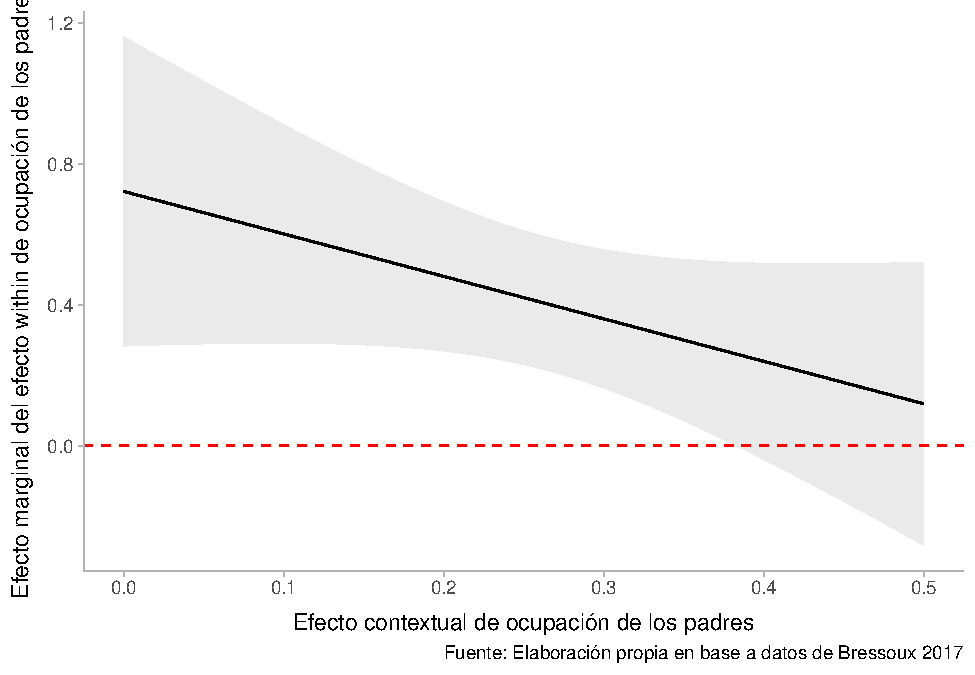
\includegraphics[width=0.8\linewidth]{02-guia_files/figure-latex/fig1-1} 

}

\caption{Efecto marginal del efecto within de ocupación padres moderado por su media grupal}\label{fig:fig1}
\end{figure}

\hypertarget{enunciado-6}{%
\section{Enunciado 6}\label{enunciado-6}}

Estime un modelo multinivel lo más parsimonioso posible para predecir el ``puntaje en la prueba de francés'' a partir de los efectos within del género, repitencia y hermanos de los estudiantes (codifique la variable hermanos como dummy, donde quienes tienen más de 1 hermano quedan asignados al 1, y quienes tienen 1 hermano o menos son la categoría de referencia).

\begin{enumerate}
\def\labelenumi{\alph{enumi})}
\tightlist
\item
  Reporte sus resultados en una tabla e interprete el intercepto fijo del modelo y el efecto within de ``repitencia'' (6 puntos).
\end{enumerate}

En la Tabla \ref{tab:table6} se presentan los resultados del modelo multinivel para el puntaje en la prueba de francés con el género, repitencia y cantidad de hermanos como covariables centrados a su media grupal (CWC). Los resultados sugieren que el efecto \emph{within} de la repitencia es negativo y estadísticamente significativo (\(\beta\) = -1.08, \(p\) \textless{} 0.001). En detalle, dentro de las clases los estudiantes que han repetido curso obtienen, en promedio, 1.08 puntos menos en la prueba de francés en comparación con quienes no han repetido, controlando por las demás variables (con estudiantes del mismo género y número de hermanos). Esta relación estadísticamente significativa con un 99,9\% de confianza. Sustantivamente, este efecto da cuenta de las diferencias individuales de la repitencia en el puntaje de francés \emph{dentro} de las clases. Esto también se debe a que un centrado CWC permite obtener un efecto ``puro'' de la relación entre dos variables de nivel individual, como es el caso (\protect\hyperlink{ref-enders_centering_2007}{Enders \& Tofighi, 2007}). Por otro lado, el intercepto del modelo es positivo pero no estadísticamente significativo (\(\beta\) = 0.02, \(p\) \textgreater{} 0.05). Este coeficiente indica el promedio del puntaje en la prueba de francés para cada clase cuando la proporción de casos para género, repitencia y hermanos es igual que la de la media grupal.

\begin{table}[h!]
\begin{center}
\scalebox{0.9}{
\begin{threeparttable}
\begin{tabular}{l c}
\toprule
 & Modelo 5 \\
\midrule
Intercepto                                       & $0.02$        \\
                                                 & $(0.07)$      \\
Mujer CWC (Ref.= Hombre)                         & $0.41^{***}$  \\
                                                 & $(0.07)$      \\
Repitencia CWC (Ref.= No repitencia)             & $-1.08^{***}$ \\
                                                 & $(0.15)$      \\
Más de un hermano CWC (Ref.= Un hermano o menos) & $0.04$        \\
                                                 & $(0.07)$      \\
\midrule
AIC                                              & $1614.34$     \\
BIC                                              & $1640.77$     \\
Log Likelihood                                   & $-801.17$     \\
Num. obs.                                        & $605$         \\
Num. groups: classe2                             & $32$          \\
Var: classe2 (Intercept)                         & $0.11$        \\
Var: Residual                                    & $0.76$        \\
\bottomrule
\end{tabular}
\begin{tablenotes}[flushleft]
\scriptsize{\item Nota: Celdas contienen coeficientes de regresión con errores estándares entre paréntesis. $^{***}p<0.001$; $^{**}p<0.01$; $^{*}p<0.05$ \\ \item Fuente: Elaboración propia en base a datos de Bressoux 2017}
\end{tablenotes}
\end{threeparttable}
}
\caption{\label{tab:table6} Modelo multinivel para puntaje en prueba de francés, género, repitencia del curso y cantidad de hermanos}
\label{table:coefficients}
\end{center}
\end{table}

\begin{enumerate}
\def\labelenumi{\alph{enumi})}
\setcounter{enumi}{1}
\tightlist
\item
  Los investigadores sostienen que el efecto del género sobre el rendimiento en francés depende de la composición de género del curso. Para evaluar esta hipótesis estime dos modelos: i) primero, uno que le permita obtener el efecto within y contextual del género, controlando por repitencia y hermanos. ii) Luego, agregue a i) una interacción entre los efectos within y contextual del género. Compare el ajuste de ambos modelos utilizando criterios estadísticos y concluya que modelo ajusta mejor a los datos (5 puntos).
\end{enumerate}

En la Tabla \ref{tab:table7} se muestran los resultados de los modelos multinivel para el puntaje en la prueba de francés según el efecto within y contextual del género, controlando por la repitencia y número de hermanos. Los resultados del modelo 6 sugieren que el efecto within del género centrado a su gran media es positivo y estadísticamente significativo (\(\beta\) = 0.41, \(p\) \textless{} 0.05), sin embargo, en el modelo 7 este coeficiente voltea su signo a negativo y deja de ser estadísticamente significativo (\(\beta\) = -0.28, \(p\) \textgreater{} 0.05). Por su parte, el efecto contextual del género es negativo pero no estadísticamente signiticativo en ambos modelos. Ahora bien, en el modelo 7 se incluye una interacción entre el efecto within y contextual del género, siendo positivo (\(\beta\) = 1.46) y estadísticamente significativo al 95\% de confianza.

\begin{table}[H]
\begin{center}
\scalebox{0.9}{
\begin{threeparttable}
\begin{tabular}{l c c}
\toprule
 & Modelo 6 & Modelo 7 \\
\midrule
Intercepto                                        & $0.09$        & $0.09$        \\
                                                  & $(0.28)$      & $(0.28)$      \\
Mujer CGM (Ref.= Hombre)                          & $0.41^{***}$  & $-0.28$       \\
                                                  & $(0.07)$      & $(0.31)$      \\
Repitencia CGM (Ref.= No repitencia)              & $-1.08^{***}$ & $-1.05^{***}$ \\
                                                  & $(0.15)$      & $(0.15)$      \\
Más de un hermano CGM (Ref.= Menos de un hermano) & $0.04$        & $0.03$        \\
                                                  & $(0.07)$      & $(0.07)$      \\
Mujer CM (Ref.= Hombre)                           & $-0.15$       & $-0.15$       \\
                                                  & $(0.58)$      & $(0.58)$      \\
Mujer CGM x Mujer CM                              &               & $1.46^{*}$    \\
                                                  &               & $(0.64)$      \\
\midrule
AIC                                               & $1615.54$     & $1615.43$     \\
BIC                                               & $1646.38$     & $1659.48$     \\
Log Likelihood                                    & $-800.77$     & $-797.71$     \\
Num. obs.                                         & $605$         & $605$         \\
Num. groups: classe2                              & $32$          & $32$          \\
Var: classe2 (Intercept)                          & $0.11$        & $0.11$        \\
Var: Residual                                     & $0.76$        & $0.76$        \\
Var: classe2 fille\_cgm                           & $$            & $0.00$        \\
Cov: classe2 (Intercept) fille\_cgm               & $$            & $0.00$        \\
\bottomrule
\end{tabular}
\begin{tablenotes}[flushleft]
\scriptsize{\item Nota: Celdas contienen coeficientes de regresión con errores estándares entre paréntesis. $^{***}p<0.001$; $^{**}p<0.01$; $^{*}p<0.05$ \\ \item Fuente: Elaboración propia en base a datos de Bressoux 2017}
\end{tablenotes}
\end{threeparttable}
}
\caption{\label{tab:table7} Modelos multinivel para puntaje en prueba de francés según efectos within y contextuales del género}
\label{table:coefficients}
\end{center}
\end{table}

En la Tabla \ref{tab:table8} se reportan los estadísticos del análisis de devianza (likelihood ratio test) para el contraste entre el Modelo 6 y 7. La prueba de razón de verosimilitud se utiliza para comparar modelos anidados y determinar cuál se ajusta mejor a los datos (\protect\hyperlink{ref-peugh_practical_2010}{Peugh, 2010}).

La hipótesis nula para esta prueba es que el efecto de la interacción entre el efecto within y contextual del género es igual a cero, mientras que la hipótesis alternativa sostiene que el efecto de la interacción es distinto de cero. Formalmente, las hipótesis son:

\[
H_0 : \beta_{1j} = 0
\]
\[
H_A : \beta_{1j} \neq 0
\]

Los resultados del análisis muestran que la prueba de razón de verosimilitud no es estadísticamente significativa, \(\chi^2\) (3) = 5.19, \(p\) = 0.2. Esto indica que el Modelo 7, que incluye la interacción entre el efecto within y contextual del género, no ajusta significativamente mejor a los datos que el Modelo 6, que no considera esta interacción. Además, el Modelo 6 presenta valores menores de AIC y BIC en comparación con el Modelo 7, lo que refuerza la idea de un mejor ajuste (\protect\hyperlink{ref-hox_multilevel_2017a}{Hox et al., 2017}). Con todo, los resultados sugieren que es no posible rechazar la \(H_0\), por lo que es preferible restringuir la interacción.

\begin{table}[!h]

\caption{\label{tab:table8}\label{tab:table8} Estadísticos de bondad de ajuste}
\centering
\begin{tabular}[t]{>{\raggedright\arraybackslash}p{2cm}rrrrrl}
\toprule
\textbf{Modelo} & \textbf{AIC} & \textbf{BIC} & \textbf{Deviance} & \textbf{X2} & \textbf{Df} & \textbf{p-value}\\
\midrule
Modelo 6 & 1604.059 & 1634.895 & 1590.059 &  &  & \\
Modelo 7 & 1604.873 & 1648.925 & 1584.873 & 5.19 & 3 & p > 0.05\\
\bottomrule
\end{tabular}
\end{table}

\begin{enumerate}
\def\labelenumi{\alph{enumi})}
\setcounter{enumi}{2}
\tightlist
\item
  Interprete sustantivamente la interacción estimada. Puede apoyarse en cálculos y/o herramientas gráficas (repórtelas).¿Qué nos dicen los datos respecto de la hipótesis sostenida por los investigadores? (7 puntos).
\end{enumerate}

Los resultados del Modelo 7 de la Tabla \ref{tab:table7}, sugieren que el efecto de la interacción entre el efecto within y contextual del género sobre el puntaje en la prueba de francés es positivo y estadísticamente significativo (\(\beta\) = 1.46, \(p\) \textless{} 0.05). Esto se respalda en la Figura \ref{fig:fig2} que muestra los efectos marginales de esta interacción. Como se aprecia, la pendiente es positiva y estadísticamente significativa cuando el efecto contextual toma valores superiores a 0.35, lo cual indica que el efecto within varía en función de la composición de género en la clase. Es decir, a medida que aumenta la proporción de mujeres en la clase (efecto contextual mayor), el efecto within de ser mujer sobre el puntaje en la prueba de francés se incrementa.

\begin{figure}

{\centering 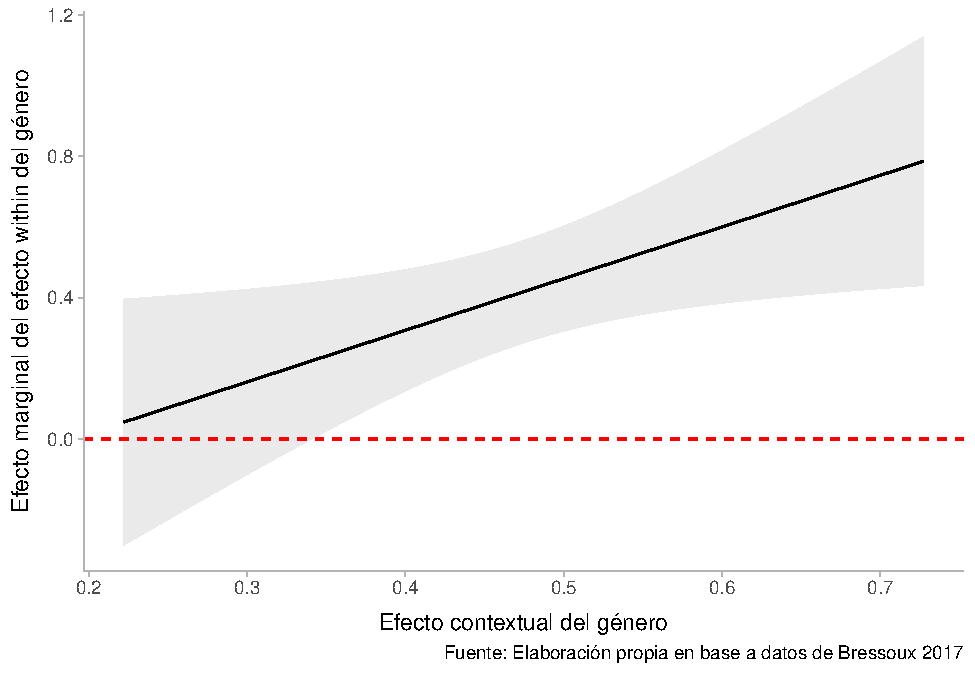
\includegraphics[width=0.8\linewidth]{02-guia_files/figure-latex/fig2-1} 

}

\caption{Efecto marginal del efecto within del género moderado por su efecto contextual}\label{fig:fig2}
\end{figure}

Sustantivamente, estos resultados indican que, en una clase donde no hay diferencias significativas entre los cursos en términos de la composición de género (efecto \emph{contextual} = 0), las mujeres obtienen, en promedio, 0.07 puntos más que los hombres en la prueba de francés. Sin embargo, conforme aumenta la proporción de mujeres en los cursos (con mayor efecto \emph{contextual}), las mujeres logran, en promedio, un puntaje de aproximadamente 0.8 puntos más alto que los hombres cuando el efecto \emph{contextual} alcanza valores cercanos a 0.727. Este resultado ilustra que el efecto de ser mujer \emph{(within)} no es constante, sino que se amplifica a medida que la representación femenina en la clase es mayor.

Alrededor de un efecto \emph{contextual} de 0.35, el intervalo de confianza para el efecto marginal del género cruza el cero, lo que indica que a partir de ese punto, el efecto \emph{within} se vuelve estadísticamente significativo. Esto sugiere que el contexto de género en la clase modera el efecto individual de ser mujer sobre el puntaje en la prueba de francés, volviéndose más fuerte y positivo conforme crece la proporción de mujeres en la clase.

Con todo, la hipótesis de los investigadores recibe apoyo: el efecto del género depende de la composición de género de la clase. Específicamente, el efecto positivo de ser mujer en el rendimiento en la prueba de francés aumenta a medida que la clase está compuesta mayoritariamente por mujeres

\hypertarget{referencias}{%
\section{Referencias}\label{referencias}}

\hypertarget{refs}{}
\begin{CSLReferences}{1}{0}
\leavevmode\vadjust pre{\hypertarget{ref-enders_centering_2007}{}}%
Enders, C. K., \& Tofighi, D. (2007). Centering predictor variables in cross-sectional multilevel models: {A} new look at an old issue. \emph{Psychological Methods}, \emph{12}(2), 121--138. \url{https://doi.org/10.1037/1082-989X.12.2.121}

\leavevmode\vadjust pre{\hypertarget{ref-finch_multilevel_2014}{}}%
Finch, W. H., Bolin, J. E., \& Kelley, K. (2014). Multilevel {Modeling Using R}.

\leavevmode\vadjust pre{\hypertarget{ref-hox_multilevel_2017a}{}}%
Hox, J., Moerbeek, M., \& Schoot, R. van de. (2017). \emph{Multilevel {Analysis}: {Techniques} and {Applications}, {Third Edition}} (3rd ed.). New York: Routledge. \url{https://doi.org/10.4324/9781315650982}

\leavevmode\vadjust pre{\hypertarget{ref-peugh_practical_2010}{}}%
Peugh, J. L. (2010). A practical guide to multilevel modeling. \emph{Journal of School Psychology}, \emph{48}(1), 85--112. \url{https://doi.org/10.1016/j.jsp.2009.09.002}

\end{CSLReferences}

\pagebreak

\hypertarget{cuxf3digo-de-r}{%
\section{Código de R}\label{cuxf3digo-de-r}}

\begin{Shaded}
\begin{Highlighting}[]
\NormalTok{knitr}\SpecialCharTok{::}\NormalTok{opts\_chunk}\SpecialCharTok{$}\FunctionTok{set}\NormalTok{(}\AttributeTok{echo =}\NormalTok{ F,}
                      \AttributeTok{warning =}\NormalTok{ F,}
                      \AttributeTok{error =}\NormalTok{ F, }
                      \AttributeTok{message =}\NormalTok{ F) }
\ControlFlowTok{if}\NormalTok{ (}\SpecialCharTok{!} \FunctionTok{require}\NormalTok{(}\StringTok{"pacman"}\NormalTok{)) }\FunctionTok{install.packages}\NormalTok{(}\StringTok{"pacman"}\NormalTok{)}

\NormalTok{pacman}\SpecialCharTok{::}\FunctionTok{p\_load}\NormalTok{(tidyverse, }
\NormalTok{               magrittr,}
\NormalTok{               sjmisc, }
\NormalTok{               sjPlot, }
\NormalTok{               lme4, }
\NormalTok{               easystats, }
\NormalTok{               influence.ME, }
\NormalTok{               broom.mixed, }
\NormalTok{               here,}
\NormalTok{               marginaleffects,}
\NormalTok{               ggeffects,}
\NormalTok{               texreg, }
\NormalTok{               ggdist,}
\NormalTok{               misty)}

\FunctionTok{options}\NormalTok{(}\AttributeTok{scipen=}\DecValTok{999}\NormalTok{)}
\FunctionTok{rm}\NormalTok{(}\AttributeTok{list =} \FunctionTok{ls}\NormalTok{())}

\NormalTok{miles }\OtherTok{\textless{}{-}} \ControlFlowTok{function}\NormalTok{(x) \{}
  \FunctionTok{format}\NormalTok{(}\FunctionTok{round}\NormalTok{(}\FunctionTok{as.numeric}\NormalTok{(x),}\DecValTok{0}\NormalTok{), }\AttributeTok{big.mark =} \StringTok{"."}\NormalTok{)}
\NormalTok{\}}

\NormalTok{decimales }\OtherTok{\textless{}{-}} \ControlFlowTok{function}\NormalTok{(x) \{}
  \FunctionTok{format}\NormalTok{(}\FunctionTok{round}\NormalTok{(}\FunctionTok{as.numeric}\NormalTok{(x), }\DecValTok{2}\NormalTok{), }\AttributeTok{decimal.mark =} \StringTok{","}\NormalTok{)}
\NormalTok{\}}

\CommentTok{\# set theme}

\FunctionTok{theme\_set}\NormalTok{(}\FunctionTok{theme\_ggdist}\NormalTok{())}

\FunctionTok{options}\NormalTok{(}\AttributeTok{knitr.kable.NA =} \StringTok{""}\NormalTok{)}
\FunctionTok{options}\NormalTok{(}\AttributeTok{knitr.table.format=}\StringTok{"latex"}\NormalTok{)}

\FunctionTok{load}\NormalTok{(}\AttributeTok{file =} \FunctionTok{here}\NormalTok{(}\StringTok{"input/data/Bressoux.RData"}\NormalTok{))}

\FunctionTok{names}\NormalTok{(Bressoux)}
\FunctionTok{glimpse}\NormalTok{(Bressoux)}

\CommentTok{\# seleccionar {-}{-}{-}{-}}

\NormalTok{db }\OtherTok{\textless{}{-}}\NormalTok{ Bressoux }\SpecialCharTok{\%\textgreater{}\%} 
\NormalTok{  dplyr}\SpecialCharTok{::}\FunctionTok{select}\NormalTok{(ecole2, classe2, numeleve, fran4, rdblt2, }
\NormalTok{                frat, fille, sup, inter, arti, empl, ouvr,}
\NormalTok{                autr, cmult) }\SpecialCharTok{\%\textgreater{}\%} 
\NormalTok{  sjlabelled}\SpecialCharTok{::}\FunctionTok{remove\_all\_labels}\NormalTok{() }\SpecialCharTok{\%\textgreater{}\%} 
\NormalTok{  janitor}\SpecialCharTok{::}\FunctionTok{clean\_names}\NormalTok{() }\SpecialCharTok{\%\textgreater{}\%} 
  \FunctionTok{as\_tibble}\NormalTok{()}
 
\CommentTok{\# filtrar: no {-}{-}{-}{-}{-} }

\CommentTok{\# recodificar y transformar: luego {-}{-}{-}{-}}

\CommentTok{\# fran4}
\NormalTok{sjmisc}\SpecialCharTok{::}\FunctionTok{descr}\NormalTok{(db}\SpecialCharTok{$}\NormalTok{fran4)}

\CommentTok{\# fille}
\FunctionTok{frq}\NormalTok{(db}\SpecialCharTok{$}\NormalTok{fille)}

\CommentTok{\# rbdlt2}
\FunctionTok{frq}\NormalTok{(db}\SpecialCharTok{$}\NormalTok{rdblt2)}

\CommentTok{\# clase multigrado}
\FunctionTok{frq}\NormalTok{(db}\SpecialCharTok{$}\NormalTok{cmult)}

\CommentTok{\# hermanos}
\FunctionTok{frq}\NormalTok{(db}\SpecialCharTok{$}\NormalTok{frat)}

\CommentTok{\# casos perdidos {-}{-}{-}{-}{-}}

\FunctionTok{colSums}\NormalTok{(}\FunctionTok{is.na}\NormalTok{(db))}

\NormalTok{db }\OtherTok{\textless{}{-}} \FunctionTok{na.omit}\NormalTok{(db)}

\CommentTok{\# Null model}
\NormalTok{model\_01 }\OtherTok{\textless{}{-}} \FunctionTok{lmer}\NormalTok{(fran4 }\SpecialCharTok{\textasciitilde{}} \DecValTok{1} \SpecialCharTok{+}\NormalTok{ (}\DecValTok{1} \SpecialCharTok{|}\NormalTok{ ecole2), }
                \AttributeTok{data =}\NormalTok{ db, }\AttributeTok{REML =}\NormalTok{ T)}
\NormalTok{model\_02 }\OtherTok{\textless{}{-}} \FunctionTok{lmer}\NormalTok{(fran4 }\SpecialCharTok{\textasciitilde{}} \DecValTok{1} \SpecialCharTok{+}\NormalTok{ (}\DecValTok{1} \SpecialCharTok{|}\NormalTok{ classe2), }
                \AttributeTok{data =}\NormalTok{ db, }\AttributeTok{REML =}\NormalTok{ T)}

\NormalTok{performance}\SpecialCharTok{::}\FunctionTok{icc}\NormalTok{(model\_01, }\AttributeTok{by\_group =}\NormalTok{ T)}
\DocumentationTok{\#\# ICC ecol2 = 0.066}
\NormalTok{performance}\SpecialCharTok{::}\FunctionTok{icc}\NormalTok{(model\_02, }\AttributeTok{by\_group =}\NormalTok{ T)}
\DocumentationTok{\#\# ICC classe2 = 0.101}

\NormalTok{ccoef }\OtherTok{\textless{}{-}} \FunctionTok{list}\NormalTok{(}
  \StringTok{"(Intercept)"} \OtherTok{=} \StringTok{"Intercepto"}\NormalTok{)}

\NormalTok{texreg}\SpecialCharTok{::}\FunctionTok{texreg}\NormalTok{(}\FunctionTok{list}\NormalTok{(model\_01, model\_02),}
               \AttributeTok{custom.model.names =} \FunctionTok{c}\NormalTok{(}\StringTok{"Modelo Nulo (ecole2)"}\NormalTok{,}
                                      \StringTok{"Modelo Nulo (classe2)"}\NormalTok{),}
               \AttributeTok{caption =} \FunctionTok{paste}\NormalTok{(}\StringTok{"(}\SpecialCharTok{\textbackslash{}\textbackslash{}}\StringTok{\#tab:table1)"}\NormalTok{,}\StringTok{"Modelos multinivel nulos con diferentes unidades de agrupación para puntaje en prueba de francés"}\NormalTok{),}
               \AttributeTok{stars =} \FunctionTok{c}\NormalTok{(}\FloatTok{0.05}\NormalTok{, }\FloatTok{0.01}\NormalTok{, }\FloatTok{0.001}\NormalTok{),}
               \AttributeTok{custom.coef.map =}\NormalTok{ ccoef,}
               \AttributeTok{custom.note =} \StringTok{"}\SpecialCharTok{\textbackslash{}\textbackslash{}}\StringTok{item Nota: Celdas contienen coeficientes de regresión con errores estándares entre paréntesis. \%stars }\SpecialCharTok{\textbackslash{}\textbackslash{}\textbackslash{}\textbackslash{}}\StringTok{ }\SpecialCharTok{\textbackslash{}\textbackslash{}}\StringTok{item Fuente: Elaboración propia en base a datos de Bressoux 2017."}\NormalTok{,}
               \AttributeTok{threeparttable =}\NormalTok{ T,}
               \AttributeTok{leading.zero =}\NormalTok{ T,}
               \AttributeTok{float.pos =} \StringTok{"h!"}\NormalTok{,}
               \AttributeTok{use.packages =}\NormalTok{ F,}
               \AttributeTok{booktabs =} \ConstantTok{TRUE}\NormalTok{,}
               \AttributeTok{scalebox =} \FloatTok{0.9}\NormalTok{)}


\CommentTok{\# Modelo lineal: cmult}
\NormalTok{model\_ols }\OtherTok{\textless{}{-}} \FunctionTok{lm}\NormalTok{(fran4 }\SpecialCharTok{\textasciitilde{}} \DecValTok{1} \SpecialCharTok{+}\NormalTok{ cmult, }\AttributeTok{data =}\NormalTok{ db)}

\CommentTok{\# Modelo 1: cmult}
\NormalTok{model\_1 }\OtherTok{\textless{}{-}} \FunctionTok{lmer}\NormalTok{(fran4 }\SpecialCharTok{\textasciitilde{}} \DecValTok{1} \SpecialCharTok{+}\NormalTok{ cmult }\SpecialCharTok{+}\NormalTok{ (}\DecValTok{1} \SpecialCharTok{|}\NormalTok{ classe2),}
                \AttributeTok{data =}\NormalTok{ db, }
                \AttributeTok{REML =}\NormalTok{ T)}


\NormalTok{ccoef }\OtherTok{\textless{}{-}} \FunctionTok{list}\NormalTok{(}
  \StringTok{"(Intercept)"} \OtherTok{=} \StringTok{"Intercepto"}\NormalTok{,}
  \AttributeTok{cmult =} \StringTok{"Curso multigrado (Ref.= Mismo grado)"}\NormalTok{)}


\NormalTok{texreg}\SpecialCharTok{::}\FunctionTok{texreg}\NormalTok{(}\FunctionTok{list}\NormalTok{(model\_ols, model\_1),}
               \AttributeTok{custom.model.names =} \FunctionTok{c}\NormalTok{(}\StringTok{"Modelo 1"}\NormalTok{,}
                                      \StringTok{"Modelo 2"}\NormalTok{),}
               \AttributeTok{caption =} \FunctionTok{paste}\NormalTok{(}\StringTok{"(}\SpecialCharTok{\textbackslash{}\textbackslash{}}\StringTok{\#tab:table2)"}\NormalTok{,}\StringTok{"Comparación de Modelos OLS y MLM para puntaje en prueba de fránces y clase multigrado"}\NormalTok{),}
               \AttributeTok{stars =} \FunctionTok{c}\NormalTok{(}\FloatTok{0.05}\NormalTok{, }\FloatTok{0.01}\NormalTok{, }\FloatTok{0.001}\NormalTok{),}
               \AttributeTok{custom.coef.map =}\NormalTok{ ccoef,}
               \AttributeTok{custom.note =} \StringTok{"}\SpecialCharTok{\textbackslash{}\textbackslash{}}\StringTok{item Nota: Celdas contienen coeficientes de regresión con errores estándares entre paréntesis. \%stars }\SpecialCharTok{\textbackslash{}\textbackslash{}\textbackslash{}\textbackslash{}}\StringTok{ }\SpecialCharTok{\textbackslash{}\textbackslash{}}\StringTok{item Fuente: Elaboración propia en base a datos de Bressoux 2017."}\NormalTok{,}
               \AttributeTok{threeparttable =}\NormalTok{ T,}
               \AttributeTok{leading.zero =}\NormalTok{ T,}
               \AttributeTok{float.pos =} \StringTok{"H"}\NormalTok{,}
               \AttributeTok{use.packages =}\NormalTok{ F,}
               \AttributeTok{booktabs =} \ConstantTok{TRUE}\NormalTok{,}
               \AttributeTok{scalebox =} \FloatTok{0.9}\NormalTok{,}
               \AttributeTok{custom.gof.rows =} \FunctionTok{list}\NormalTok{(}\StringTok{"Estimador"} \OtherTok{=} \FunctionTok{c}\NormalTok{(}\StringTok{"OLS"}\NormalTok{, }\StringTok{"MLM"}\NormalTok{)))}


\NormalTok{var\_comp }\OtherTok{\textless{}{-}} \FunctionTok{as.data.frame}\NormalTok{(}\FunctionTok{VarCorr}\NormalTok{(model\_1))}
\NormalTok{var\_resid }\OtherTok{\textless{}{-}}\NormalTok{ var\_comp}\SpecialCharTok{$}\NormalTok{vcov[}\DecValTok{2}\NormalTok{]}
\NormalTok{var\_bet }\OtherTok{\textless{}{-}}\NormalTok{ var\_comp}\SpecialCharTok{$}\NormalTok{vcov[}\DecValTok{1}\NormalTok{]}

\NormalTok{grupos }\OtherTok{\textless{}{-}}\NormalTok{ db }\SpecialCharTok{\%\textgreater{}\%}  
  \FunctionTok{group\_by}\NormalTok{(classe2) }\SpecialCharTok{\%\textgreater{}\%} 
  \FunctionTok{summarise}\NormalTok{(}\AttributeTok{nj=}\FunctionTok{n}\NormalTok{(), }
            \AttributeTok{fran4\_j =} \FunctionTok{mean}\NormalTok{(fran4, }\AttributeTok{na.rm =}\NormalTok{ T), }
            \AttributeTok{cmult\_j =} \FunctionTok{mean}\NormalTok{(cmult, }\AttributeTok{na.rm =}\NormalTok{ T))}

\NormalTok{grupos}\SpecialCharTok{$}\NormalTok{Vj }\OtherTok{\textless{}{-}}\NormalTok{ var\_resid }\SpecialCharTok{/}\NormalTok{grupos}\SpecialCharTok{$}\NormalTok{nj}
\NormalTok{grupos}\SpecialCharTok{$}\NormalTok{Deltaj }\OtherTok{\textless{}{-}}\NormalTok{ grupos}\SpecialCharTok{$}\NormalTok{Vj }\SpecialCharTok{+}\NormalTok{ var\_bet}

\NormalTok{fran4\_jp }\OtherTok{\textless{}{-}} \FunctionTok{sum}\NormalTok{(grupos}\SpecialCharTok{$}\NormalTok{fran4\_j}\SpecialCharTok{*}\NormalTok{grupos}\SpecialCharTok{$}\NormalTok{Deltaj}\SpecialCharTok{\^{}{-}}\DecValTok{1}\NormalTok{)}\SpecialCharTok{/}\FunctionTok{sum}\NormalTok{(grupos}\SpecialCharTok{$}\NormalTok{Deltaj}\SpecialCharTok{\^{}{-}}\DecValTok{1}\NormalTok{)}

\NormalTok{cmult\_jp }\OtherTok{\textless{}{-}} \FunctionTok{sum}\NormalTok{(grupos}\SpecialCharTok{$}\NormalTok{cmult\_j}\SpecialCharTok{*}\NormalTok{grupos}\SpecialCharTok{$}\NormalTok{Deltaj}\SpecialCharTok{\^{}{-}}\DecValTok{1}\NormalTok{)}\SpecialCharTok{/}\FunctionTok{sum}\NormalTok{(grupos}\SpecialCharTok{$}\NormalTok{Deltaj}\SpecialCharTok{\^{}{-}}\DecValTok{1}\NormalTok{)}

\NormalTok{beta01\_m }\OtherTok{\textless{}{-}} \FunctionTok{sum}\NormalTok{(grupos}\SpecialCharTok{$}\NormalTok{Deltaj}\SpecialCharTok{\^{}{-}}\DecValTok{1}\SpecialCharTok{*}\NormalTok{(grupos}\SpecialCharTok{$}\NormalTok{cmult\_j }\SpecialCharTok{{-}}\NormalTok{ cmult\_jp)}\SpecialCharTok{*}\NormalTok{(grupos}\SpecialCharTok{$}\NormalTok{fran4\_j }\SpecialCharTok{{-}}\NormalTok{ fran4\_jp))}\SpecialCharTok{/} 
\NormalTok{  (}\FunctionTok{sum}\NormalTok{(grupos}\SpecialCharTok{$}\NormalTok{Deltaj}\SpecialCharTok{\^{}{-}}\DecValTok{1}\SpecialCharTok{*}\NormalTok{(grupos}\SpecialCharTok{$}\NormalTok{cmult\_j }\SpecialCharTok{{-}}\NormalTok{ cmult\_jp)}\SpecialCharTok{\^{}}\DecValTok{2}\NormalTok{))}

\NormalTok{beta01\_m}
\CommentTok{\# Centrado GMC}
\NormalTok{db }\OtherTok{\textless{}{-}}\NormalTok{ db }\SpecialCharTok{\%\textgreater{}\%} 
  \FunctionTok{mutate}\NormalTok{(}\AttributeTok{cmult\_mean =} \FunctionTok{mean}\NormalTok{(cmult, }\AttributeTok{na.rm =}\NormalTok{ T),}
         \AttributeTok{cmult\_cgm =}\NormalTok{ cmult }\SpecialCharTok{{-}}\NormalTok{ cmult\_mean,}
         \AttributeTok{fille\_mean =} \FunctionTok{mean}\NormalTok{(fille, }\AttributeTok{na.rm =}\NormalTok{ T),}
         \AttributeTok{fille\_cgm =}\NormalTok{ fille }\SpecialCharTok{{-}}\NormalTok{ fille\_mean,}
         \AttributeTok{rdblt2\_mean =} \FunctionTok{mean}\NormalTok{(rdblt2, }\AttributeTok{na.rm =}\NormalTok{ T),}
         \AttributeTok{rdblt2\_cgm =}\NormalTok{ rdblt2 }\SpecialCharTok{{-}}\NormalTok{ rdblt2\_mean)}

\FunctionTok{summary}\NormalTok{(db}\SpecialCharTok{$}\NormalTok{cmult\_cgm)}
\NormalTok{datawizard}\SpecialCharTok{::}\FunctionTok{center}\NormalTok{(db}\SpecialCharTok{$}\NormalTok{cmult) }\CommentTok{\# ok}

\NormalTok{model\_2 }\OtherTok{\textless{}{-}} \FunctionTok{lmer}\NormalTok{(fran4 }\SpecialCharTok{\textasciitilde{}} \DecValTok{1} \SpecialCharTok{+}\NormalTok{ cmult\_cgm }\SpecialCharTok{+}\NormalTok{ fille\_cgm }\SpecialCharTok{+}
\NormalTok{                rdblt2\_cgm }\SpecialCharTok{+}\NormalTok{ (}\DecValTok{1} \SpecialCharTok{|}\NormalTok{ classe2),}
                \AttributeTok{data =}\NormalTok{ db, }
                \AttributeTok{REML =}\NormalTok{ T)}


\NormalTok{ccoef }\OtherTok{\textless{}{-}} \FunctionTok{list}\NormalTok{(}
  \StringTok{"(Intercept)"} \OtherTok{=} \StringTok{"Intercepto"}\NormalTok{,}
  \AttributeTok{cmult\_cgm =} \StringTok{"Curso multigrado CGM (Ref.= Mismo grado)"}\NormalTok{,}
  \AttributeTok{fille\_cgm =} \StringTok{"Mujer CGM (Ref.= Hombre)"}\NormalTok{,}
  \AttributeTok{rdblt2\_cgm =} \StringTok{"Repitencia CGM (Ref.= No repitencia)"}\NormalTok{)}


\NormalTok{texreg}\SpecialCharTok{::}\FunctionTok{texreg}\NormalTok{(}\FunctionTok{list}\NormalTok{(model\_2),}
               \AttributeTok{custom.model.names =} \FunctionTok{c}\NormalTok{(}\StringTok{"Modelo 3"}\NormalTok{),}
               \AttributeTok{caption =} \FunctionTok{paste}\NormalTok{(}\StringTok{"(}\SpecialCharTok{\textbackslash{}\textbackslash{}}\StringTok{\#tab:table3)"}\NormalTok{,}\StringTok{"Modelo multinivel para puntaje en prueba de francés, género y repitencia del curso"}\NormalTok{),}
               \AttributeTok{stars =} \FunctionTok{c}\NormalTok{(}\FloatTok{0.05}\NormalTok{, }\FloatTok{0.01}\NormalTok{, }\FloatTok{0.001}\NormalTok{),}
               \AttributeTok{custom.coef.map =}\NormalTok{ ccoef,}
               \AttributeTok{custom.note =} \StringTok{"}\SpecialCharTok{\textbackslash{}\textbackslash{}}\StringTok{item Nota: Celdas contienen coeficientes de regresión con errores estándares entre paréntesis. \%stars }\SpecialCharTok{\textbackslash{}\textbackslash{}\textbackslash{}\textbackslash{}}\StringTok{ }\SpecialCharTok{\textbackslash{}\textbackslash{}}\StringTok{item Fuente: Elaboración propia en base a datos de Bressoux 2017."}\NormalTok{,}
               \AttributeTok{threeparttable =}\NormalTok{ T,}
               \AttributeTok{leading.zero =}\NormalTok{ T,}
               \AttributeTok{float.pos =} \StringTok{"H"}\NormalTok{,}
               \AttributeTok{use.packages =}\NormalTok{ F,}
               \AttributeTok{booktabs =} \ConstantTok{TRUE}\NormalTok{,}
               \AttributeTok{scalebox =} \FloatTok{0.9}\NormalTok{)}


\CommentTok{\# employed}
\FunctionTok{frq}\NormalTok{(db}\SpecialCharTok{$}\NormalTok{sup)}
\FunctionTok{frq}\NormalTok{(db}\SpecialCharTok{$}\NormalTok{inter)}

\NormalTok{db }\OtherTok{\textless{}{-}}\NormalTok{ db }\SpecialCharTok{\%\textgreater{}\%} 
  \FunctionTok{mutate}\NormalTok{(}\AttributeTok{p\_profint =} \FunctionTok{if\_else}\NormalTok{(sup }\SpecialCharTok{==} \DecValTok{1} \SpecialCharTok{|}\NormalTok{ inter }\SpecialCharTok{==} \DecValTok{1}\NormalTok{, }\DecValTok{1}\NormalTok{, }\DecValTok{0}\NormalTok{))}

\NormalTok{db}\SpecialCharTok{$}\NormalTok{gm\_p\_profint }\OtherTok{\textless{}{-}} \FunctionTok{mean}\NormalTok{(db}\SpecialCharTok{$}\NormalTok{p\_profint, }\AttributeTok{use=}\StringTok{"complete.obs"}\NormalTok{)}
\NormalTok{db}\SpecialCharTok{$}\NormalTok{p\_profint\_cgm }\OtherTok{\textless{}{-}}\NormalTok{ db}\SpecialCharTok{$}\NormalTok{p\_profint }\SpecialCharTok{{-}}\NormalTok{ db}\SpecialCharTok{$}\NormalTok{gm\_p\_profint}
\NormalTok{db }\OtherTok{\textless{}{-}}\NormalTok{ db }\SpecialCharTok{\%\textgreater{}\%} \FunctionTok{group\_by}\NormalTok{(classe2) }\SpecialCharTok{\%\textgreater{}\%}
  \FunctionTok{mutate}\NormalTok{(}\AttributeTok{cm\_p\_profint =} \FunctionTok{mean}\NormalTok{(p\_profint))}

\NormalTok{model\_3 }\OtherTok{\textless{}{-}} \FunctionTok{lmer}\NormalTok{(fran4 }\SpecialCharTok{\textasciitilde{}}\NormalTok{ cmult\_cgm }\SpecialCharTok{+}\NormalTok{ fille\_cgm }\SpecialCharTok{+} 
\NormalTok{                  rdblt2\_cgm }\SpecialCharTok{+}\NormalTok{ p\_profint\_cgm }\SpecialCharTok{+} 
\NormalTok{                  cm\_p\_profint }\SpecialCharTok{+}\NormalTok{ (}\DecValTok{1}\SpecialCharTok{|}\NormalTok{classe2), }
                \AttributeTok{data =}\NormalTok{ db, }
                \AttributeTok{REML =}\NormalTok{ T)}

\NormalTok{ccoef }\OtherTok{\textless{}{-}} \FunctionTok{list}\NormalTok{(}
  \StringTok{"(Intercept)"} \OtherTok{=} \StringTok{"Intercepto"}\NormalTok{,}
  \AttributeTok{cmult\_cgm =} \StringTok{"Curso multigrado CGM (Ref.= Mismo grado)"}\NormalTok{,}
  \AttributeTok{fille\_cgm =} \StringTok{"Mujer CGM (Ref.= Hombre)"}\NormalTok{,}
  \AttributeTok{rdblt2\_cgm =} \StringTok{"Repitencia CGM (Ref.= No repitencia)"}\NormalTok{,}
  \AttributeTok{p\_profint\_cgm =} \StringTok{"Padres con P/I CGM (Ref.= Sin padres P/I)"}\NormalTok{,}
  \AttributeTok{cm\_p\_profint =} \StringTok{"Padres con P/I CM (Ref.= Sin padres P/I)"}\NormalTok{)}


\NormalTok{texreg}\SpecialCharTok{::}\FunctionTok{texreg}\NormalTok{(}\FunctionTok{list}\NormalTok{(model\_3),}
               \AttributeTok{custom.model.names =} \FunctionTok{c}\NormalTok{(}\StringTok{"Modelo 4"}\NormalTok{),}
               \AttributeTok{caption =} \FunctionTok{paste}\NormalTok{(}\StringTok{"(}\SpecialCharTok{\textbackslash{}\textbackslash{}}\StringTok{\#tab:table4)"}\NormalTok{,}\StringTok{"Modelo multinivel para puntaje en prueba de francés, género, repitencia del curso y padres con ocupaciones profesionales o intermedias"}\NormalTok{),}
               \AttributeTok{stars =} \FunctionTok{c}\NormalTok{(}\FloatTok{0.05}\NormalTok{, }\FloatTok{0.01}\NormalTok{, }\FloatTok{0.001}\NormalTok{),}
               \AttributeTok{custom.coef.map =}\NormalTok{ ccoef,}
               \AttributeTok{custom.note =} \StringTok{"}\SpecialCharTok{\textbackslash{}\textbackslash{}}\StringTok{item Nota: Celdas contienen coeficientes de regresión con errores estándares entre paréntesis. \%stars }\SpecialCharTok{\textbackslash{}\textbackslash{}\textbackslash{}\textbackslash{}}\StringTok{ }\SpecialCharTok{\textbackslash{}\textbackslash{}}\StringTok{item Fuente: Elaboración propia en base a datos de Bressoux 2017. }\SpecialCharTok{\textbackslash{}\textbackslash{}\textbackslash{}\textbackslash{}}\StringTok{ }\SpecialCharTok{\textbackslash{}\textbackslash{}}\StringTok{item P/I = Ocupaciones profesionales o intermedias"}\NormalTok{,}
               \AttributeTok{threeparttable =}\NormalTok{ T,}
               \AttributeTok{leading.zero =}\NormalTok{ T,}
               \AttributeTok{float.pos =} \StringTok{"H"}\NormalTok{,}
               \AttributeTok{use.packages =}\NormalTok{ F,}
               \AttributeTok{booktabs =} \ConstantTok{TRUE}\NormalTok{,}
               \AttributeTok{scalebox =} \FloatTok{0.9}\NormalTok{)}



\NormalTok{model\_4 }\OtherTok{\textless{}{-}} \FunctionTok{lmer}\NormalTok{(fran4 }\SpecialCharTok{\textasciitilde{}}\NormalTok{ cmult\_cgm }\SpecialCharTok{+}\NormalTok{ fille\_cgm }\SpecialCharTok{+} 
\NormalTok{                  rdblt2\_cgm }\SpecialCharTok{+}\NormalTok{ p\_profint\_cgm }\SpecialCharTok{*} 
\NormalTok{                  cm\_p\_profint }\SpecialCharTok{+}\NormalTok{ (p\_profint\_cgm }\SpecialCharTok{+} \DecValTok{1}\SpecialCharTok{|}\NormalTok{classe2), }
                \AttributeTok{data =}\NormalTok{ db,}
                \AttributeTok{REML =}\NormalTok{ T)}

\NormalTok{ccoef }\OtherTok{\textless{}{-}} \FunctionTok{list}\NormalTok{(}
  \StringTok{"(Intercept)"} \OtherTok{=} \StringTok{"Intercepto"}\NormalTok{,}
  \AttributeTok{cmult\_cgm =} \StringTok{"Curso multigrado CGM (Ref.= Mismo grado)"}\NormalTok{,}
  \AttributeTok{fille\_cgm =} \StringTok{"Mujer CGM (Ref.= Hombre)"}\NormalTok{,}
  \AttributeTok{rdblt2\_cgm =} \StringTok{"Repitencia CGM (Ref.= No repitencia)"}\NormalTok{,}
  \AttributeTok{p\_profint\_cgm =} \StringTok{"Padres con P/I CGM (Ref.= Sin padres P/I)"}\NormalTok{,}
  \AttributeTok{cm\_p\_profint =} \StringTok{"Padres con P/I CM (Ref.= Sin padres P/I)"}\NormalTok{,}
  \StringTok{"p\_profint\_cgm:cm\_p\_profint"} \OtherTok{=} \StringTok{"Padres con P/I CGM x Padres con P/I CM"}\NormalTok{)}


\NormalTok{texreg}\SpecialCharTok{::}\FunctionTok{texreg}\NormalTok{(}\FunctionTok{list}\NormalTok{(model\_4),}
               \AttributeTok{custom.model.names =} \FunctionTok{c}\NormalTok{(}\StringTok{"Modelo 4"}\NormalTok{),}
               \AttributeTok{caption =} \FunctionTok{paste}\NormalTok{(}\StringTok{"(}\SpecialCharTok{\textbackslash{}\textbackslash{}}\StringTok{\#tab:table5)"}\NormalTok{,}\StringTok{"Modelo multinivel para puntaje en prueba de francés, género, repitencia del curso y padres con ocupaciones profesionales o intermedias con interacción"}\NormalTok{),}
               \AttributeTok{stars =} \FunctionTok{c}\NormalTok{(}\FloatTok{0.05}\NormalTok{, }\FloatTok{0.01}\NormalTok{, }\FloatTok{0.001}\NormalTok{),}
               \AttributeTok{custom.coef.map =}\NormalTok{ ccoef,}
               \AttributeTok{custom.note =} \StringTok{"}\SpecialCharTok{\textbackslash{}\textbackslash{}}\StringTok{item Nota: Celdas contienen coeficientes de regresión con errores estándares entre paréntesis. \%stars }\SpecialCharTok{\textbackslash{}\textbackslash{}\textbackslash{}\textbackslash{}}\StringTok{ }\SpecialCharTok{\textbackslash{}\textbackslash{}}\StringTok{item Fuente: Elaboración propia en base a datos de Bressoux 2017. }\SpecialCharTok{\textbackslash{}\textbackslash{}\textbackslash{}\textbackslash{}}\StringTok{ }\SpecialCharTok{\textbackslash{}\textbackslash{}}\StringTok{item P/I = Ocupaciones profesionales o intermedias"}\NormalTok{,}
               \AttributeTok{threeparttable =}\NormalTok{ T,}
               \AttributeTok{leading.zero =}\NormalTok{ T,}
               \AttributeTok{float.pos =} \StringTok{"H"}\NormalTok{,}
               \AttributeTok{use.packages =}\NormalTok{ F,}
               \AttributeTok{booktabs =} \ConstantTok{TRUE}\NormalTok{,}
               \AttributeTok{scalebox =} \FloatTok{0.9}\NormalTok{)}



\FunctionTok{plot\_slopes}\NormalTok{(model\_4, }
            \AttributeTok{variables =} \StringTok{"p\_profint\_cgm"}\NormalTok{, }
            \AttributeTok{condition =} \StringTok{"cm\_p\_profint"}\NormalTok{,}
            \AttributeTok{conf\_level =}\NormalTok{ .}\DecValTok{95}\NormalTok{,}
            \AttributeTok{re.form =} \ConstantTok{NA}\NormalTok{) }\SpecialCharTok{+}
  \FunctionTok{geom\_hline}\NormalTok{(}\AttributeTok{yintercept =} \DecValTok{0}\NormalTok{, }
             \AttributeTok{color =} \StringTok{"red"}\NormalTok{, }
             \AttributeTok{linetype =} \StringTok{"dashed"}\NormalTok{) }\SpecialCharTok{+}
  \FunctionTok{labs}\NormalTok{(}\AttributeTok{y =} \StringTok{"Efecto marginal del efecto within de ocupación de los padres"}\NormalTok{,}
       \AttributeTok{x =} \StringTok{"Efecto contextual de ocupación de los padres"}\NormalTok{,}
       \AttributeTok{caption =} \StringTok{"Fuente: Elaboración propia en base a datos de Bressoux 2017"}\NormalTok{,}
       \AttributeTok{title =} \ConstantTok{NULL}\NormalTok{)}

\NormalTok{db }\SpecialCharTok{\%\textless{}\textgreater{}\%}
  \FunctionTok{mutate}\NormalTok{(}\AttributeTok{frat =} \FunctionTok{case\_when}\NormalTok{(frat }\SpecialCharTok{\textgreater{}} \DecValTok{1} \SpecialCharTok{\textasciitilde{}} \DecValTok{1}\NormalTok{,}
\NormalTok{                          frat }\SpecialCharTok{\textless{}=} \DecValTok{1} \SpecialCharTok{\textasciitilde{}} \DecValTok{0}\NormalTok{))}

\NormalTok{db }\SpecialCharTok{\%\textless{}\textgreater{}\%} 
  \FunctionTok{group\_by}\NormalTok{(classe2) }\SpecialCharTok{\%\textgreater{}\%} 
  \FunctionTok{mutate}\NormalTok{(}\AttributeTok{fille\_mean =} \FunctionTok{mean}\NormalTok{(fille, }\AttributeTok{na.rm =}\NormalTok{ T),}
         \AttributeTok{fille\_cwc =}\NormalTok{ fille }\SpecialCharTok{{-}}\NormalTok{ fille\_mean,}
         \AttributeTok{rdblt2\_mean =} \FunctionTok{mean}\NormalTok{(rdblt2, }\AttributeTok{na.rm =}\NormalTok{ T),}
         \AttributeTok{rdblt2\_cwc =}\NormalTok{ rdblt2 }\SpecialCharTok{{-}}\NormalTok{ rdblt2\_mean,}
         \AttributeTok{frat\_mean =} \FunctionTok{mean}\NormalTok{(frat, }\AttributeTok{na.rm =}\NormalTok{ T),}
         \AttributeTok{frat\_cwc =}\NormalTok{ frat }\SpecialCharTok{{-}}\NormalTok{ frat\_mean)}

\NormalTok{model\_5 }\OtherTok{\textless{}{-}} \FunctionTok{lmer}\NormalTok{(fran4 }\SpecialCharTok{\textasciitilde{}}\NormalTok{ fille\_cwc }\SpecialCharTok{+}\NormalTok{ rdblt2\_cwc }\SpecialCharTok{+}\NormalTok{ frat\_cwc }\SpecialCharTok{+}\NormalTok{ (}\DecValTok{1}\SpecialCharTok{|}\NormalTok{classe2), }
                \AttributeTok{data =}\NormalTok{ db,}
                \AttributeTok{REML =}\NormalTok{ T)}

\NormalTok{ccoef }\OtherTok{\textless{}{-}} \FunctionTok{list}\NormalTok{(}
  \StringTok{"(Intercept)"} \OtherTok{=} \StringTok{"Intercepto"}\NormalTok{,}
  \AttributeTok{fille\_cwc =} \StringTok{"Mujer CWC (Ref.= Hombre)"}\NormalTok{,}
  \AttributeTok{rdblt2\_cwc =} \StringTok{"Repitencia CWC (Ref.= No repitencia)"}\NormalTok{,}
  \AttributeTok{frat\_cwc =} \StringTok{"Más de un hermano CWC (Ref.= Un hermano o menos)"}\NormalTok{)}


\NormalTok{texreg}\SpecialCharTok{::}\FunctionTok{texreg}\NormalTok{(}\FunctionTok{list}\NormalTok{(model\_5),}
               \AttributeTok{custom.model.names =} \FunctionTok{c}\NormalTok{(}\StringTok{"Modelo 5"}\NormalTok{),}
               \AttributeTok{caption =} \FunctionTok{paste}\NormalTok{(}\StringTok{"(}\SpecialCharTok{\textbackslash{}\textbackslash{}}\StringTok{\#tab:table6)"}\NormalTok{,}\StringTok{"Modelo multinivel para puntaje en prueba de francés, género, repitencia del curso y cantidad de hermanos"}\NormalTok{),}
               \AttributeTok{stars =} \FunctionTok{c}\NormalTok{(}\FloatTok{0.05}\NormalTok{, }\FloatTok{0.01}\NormalTok{, }\FloatTok{0.001}\NormalTok{),}
               \AttributeTok{custom.coef.map =}\NormalTok{ ccoef,}
               \AttributeTok{custom.note =} \StringTok{"}\SpecialCharTok{\textbackslash{}\textbackslash{}}\StringTok{item Nota: Celdas contienen coeficientes de regresión con errores estándares entre paréntesis. \%stars }\SpecialCharTok{\textbackslash{}\textbackslash{}\textbackslash{}\textbackslash{}}\StringTok{ }\SpecialCharTok{\textbackslash{}\textbackslash{}}\StringTok{item Fuente: Elaboración propia en base a datos de Bressoux 2017"}\NormalTok{,}
               \AttributeTok{threeparttable =}\NormalTok{ T,}
               \AttributeTok{leading.zero =}\NormalTok{ T,}
               \AttributeTok{float.pos =} \StringTok{"h!"}\NormalTok{,}
               \AttributeTok{use.packages =}\NormalTok{ F,}
               \AttributeTok{booktabs =} \ConstantTok{TRUE}\NormalTok{,}
               \AttributeTok{scalebox =} \FloatTok{0.9}\NormalTok{)}



\NormalTok{db }\SpecialCharTok{\%\textless{}\textgreater{}\%} 
  \FunctionTok{mutate}\NormalTok{(}\AttributeTok{fille\_mean =} \FunctionTok{mean}\NormalTok{(fille, }\AttributeTok{na.rm =}\NormalTok{ T),}
         \AttributeTok{fille\_cgm =}\NormalTok{ fille }\SpecialCharTok{{-}}\NormalTok{ fille\_mean,}
         \AttributeTok{rdblt2\_mean =} \FunctionTok{mean}\NormalTok{(rdblt2, }\AttributeTok{na.rm =}\NormalTok{ T),}
         \AttributeTok{rdblt2\_cgm =}\NormalTok{ rdblt2 }\SpecialCharTok{{-}}\NormalTok{ rdblt2\_mean,}
         \AttributeTok{frat\_mean =} \FunctionTok{mean}\NormalTok{(frat, }\AttributeTok{na.rm =}\NormalTok{ T),}
         \AttributeTok{frat\_cgm =}\NormalTok{ frat }\SpecialCharTok{{-}}\NormalTok{ frat\_mean)}

\NormalTok{db }\SpecialCharTok{\%\textless{}\textgreater{}\%} 
  \FunctionTok{group\_by}\NormalTok{(classe2) }\SpecialCharTok{\%\textgreater{}\%} 
  \FunctionTok{mutate}\NormalTok{(}\AttributeTok{cm\_fille =} \FunctionTok{mean}\NormalTok{(fille, }\AttributeTok{na.rm =}\NormalTok{ T))}

\NormalTok{model\_6 }\OtherTok{\textless{}{-}} \FunctionTok{lmer}\NormalTok{(fran4 }\SpecialCharTok{\textasciitilde{}}\NormalTok{ fille\_cgm }\SpecialCharTok{+}\NormalTok{ rdblt2\_cgm }\SpecialCharTok{+}\NormalTok{ frat\_cgm }\SpecialCharTok{+}\NormalTok{ cm\_fille }\SpecialCharTok{+}\NormalTok{ (}\DecValTok{1}\SpecialCharTok{|}\NormalTok{classe2), }
                \AttributeTok{data =}\NormalTok{ db,}
                \AttributeTok{REML =}\NormalTok{ T)}

\NormalTok{model\_7 }\OtherTok{\textless{}{-}} \FunctionTok{lmer}\NormalTok{(fran4 }\SpecialCharTok{\textasciitilde{}}\NormalTok{ fille\_cgm }\SpecialCharTok{+}\NormalTok{ rdblt2\_cgm }\SpecialCharTok{+}\NormalTok{ frat\_cgm }\SpecialCharTok{+}\NormalTok{ cm\_fille }\SpecialCharTok{+} 
\NormalTok{                  fille\_cgm}\SpecialCharTok{*}\NormalTok{cm\_fille }\SpecialCharTok{+}\NormalTok{ (fille\_cgm }\SpecialCharTok{+} \DecValTok{1}\SpecialCharTok{|}\NormalTok{classe2), }
                \AttributeTok{data =}\NormalTok{ db,}
                \AttributeTok{REML =}\NormalTok{ T)}

\NormalTok{ccoef }\OtherTok{\textless{}{-}} \FunctionTok{list}\NormalTok{(}
  \StringTok{"(Intercept)"} \OtherTok{=} \StringTok{"Intercepto"}\NormalTok{,}
  \AttributeTok{fille\_cgm =} \StringTok{"Mujer CGM (Ref.= Hombre)"}\NormalTok{,}
  \AttributeTok{rdblt2\_cgm =} \StringTok{"Repitencia CGM (Ref.= No repitencia)"}\NormalTok{,}
  \AttributeTok{frat\_cgm =} \StringTok{"Más de un hermano CGM (Ref.= Menos de un hermano)"}\NormalTok{,}
  \AttributeTok{cm\_fille =} \StringTok{"Mujer CM (Ref.= Hombre)"}\NormalTok{,}
  \StringTok{"fille\_cgm:cm\_fille"} \OtherTok{=} \StringTok{"Mujer CGM x Mujer CM"}\NormalTok{)}

\NormalTok{texreg}\SpecialCharTok{::}\FunctionTok{texreg}\NormalTok{(}\FunctionTok{list}\NormalTok{(model\_6, model\_7),}
               \AttributeTok{custom.model.names =} \FunctionTok{c}\NormalTok{(}\StringTok{"Modelo 6"}\NormalTok{, }\StringTok{"Modelo 7"}\NormalTok{),}
               \AttributeTok{caption =} \FunctionTok{paste}\NormalTok{(}\StringTok{"(}\SpecialCharTok{\textbackslash{}\textbackslash{}}\StringTok{\#tab:table7)"}\NormalTok{,}\StringTok{"Modelos multinivel para puntaje en prueba de francés según efectos within y contextuales del género"}\NormalTok{),}
               \AttributeTok{stars =} \FunctionTok{c}\NormalTok{(}\FloatTok{0.05}\NormalTok{, }\FloatTok{0.01}\NormalTok{, }\FloatTok{0.001}\NormalTok{),}
               \AttributeTok{custom.coef.map =}\NormalTok{ ccoef,}
               \AttributeTok{custom.note =} \StringTok{"}\SpecialCharTok{\textbackslash{}\textbackslash{}}\StringTok{item Nota: Celdas contienen coeficientes de regresión con errores estándares entre paréntesis. \%stars }\SpecialCharTok{\textbackslash{}\textbackslash{}\textbackslash{}\textbackslash{}}\StringTok{ }\SpecialCharTok{\textbackslash{}\textbackslash{}}\StringTok{item Fuente: Elaboración propia en base a datos de Bressoux 2017"}\NormalTok{,}
               \AttributeTok{threeparttable =}\NormalTok{ T,}
               \AttributeTok{leading.zero =}\NormalTok{ T,}
               \AttributeTok{float.pos =} \StringTok{"H"}\NormalTok{,}
               \AttributeTok{use.packages =}\NormalTok{ F,}
               \AttributeTok{booktabs =} \ConstantTok{TRUE}\NormalTok{,}
               \AttributeTok{scalebox =} \FloatTok{0.9}\NormalTok{)}



\NormalTok{res\_fit1 }\OtherTok{\textless{}{-}} \FunctionTok{anova}\NormalTok{(model\_6, model\_7)}

\NormalTok{fit\_tab }\OtherTok{\textless{}{-}}\NormalTok{ res\_fit1[}\FunctionTok{c}\NormalTok{(}\DecValTok{2}\NormalTok{,}\DecValTok{3}\NormalTok{,}\DecValTok{5}\NormalTok{,}\DecValTok{6}\NormalTok{,}\DecValTok{7}\NormalTok{,}\DecValTok{8}\NormalTok{)] }\SpecialCharTok{\%\textgreater{}\%} \FunctionTok{as\_tibble}\NormalTok{(.)}

\NormalTok{fit\_tab}\SpecialCharTok{$}\NormalTok{mod }\OtherTok{\textless{}{-}} \FunctionTok{c}\NormalTok{(}\StringTok{"Modelo 6"}\NormalTok{, }\StringTok{"Modelo 7"}\NormalTok{)}

\NormalTok{fit\_tab}\SpecialCharTok{$}\NormalTok{p }\OtherTok{\textless{}{-}} \FunctionTok{if\_else}\NormalTok{(fit\_tab}\SpecialCharTok{$}\StringTok{\textasciigrave{}}\AttributeTok{Pr(\textgreater{}Chisq)}\StringTok{\textasciigrave{}} \SpecialCharTok{\textless{}} \FloatTok{0.05}\NormalTok{, }\StringTok{"p \textless{} 0.05 *"}\NormalTok{, }\StringTok{"p \textgreater{} 0.05"}\NormalTok{)}

\NormalTok{fit\_tab}\SpecialCharTok{$}\NormalTok{Chisq }\OtherTok{\textless{}{-}} \FunctionTok{round}\NormalTok{(fit\_tab}\SpecialCharTok{$}\NormalTok{Chisq, }\AttributeTok{digits =} \DecValTok{2}\NormalTok{)}

\NormalTok{fit\_tab }\OtherTok{\textless{}{-}}\NormalTok{ fit\_tab }\SpecialCharTok{\%\textgreater{}\%} 
\NormalTok{  dplyr}\SpecialCharTok{::}\FunctionTok{select}\NormalTok{(mod, AIC, BIC, deviance, Chisq, Df, p)}

\NormalTok{colnames }\OtherTok{\textless{}{-}} \FunctionTok{c}\NormalTok{(}\StringTok{"Modelo"}\NormalTok{, }\StringTok{"AIC"}\NormalTok{, }\StringTok{"BIC"}\NormalTok{, }\StringTok{"Deviance"}\NormalTok{, }\StringTok{"X2"}\NormalTok{, }\StringTok{"Df"}\NormalTok{, }\StringTok{"p{-}value"}\NormalTok{)}

\NormalTok{fit\_tab }\OtherTok{\textless{}{-}}\NormalTok{ kableExtra}\SpecialCharTok{::}\FunctionTok{kable}\NormalTok{(fit\_tab, }
                             \AttributeTok{format =} \StringTok{"latex"}\NormalTok{, }
                             \AttributeTok{col.names =}\NormalTok{ colnames,}
                             \AttributeTok{row.names =}\NormalTok{ F,}
                             \AttributeTok{booktabs =}\NormalTok{ T, }
                             \AttributeTok{caption =} \FunctionTok{paste}\NormalTok{(}\StringTok{"(}\SpecialCharTok{\textbackslash{}\textbackslash{}}\StringTok{\#tab:table8)"}\NormalTok{,}\StringTok{"Estadísticos de bondad de ajuste"}\NormalTok{),) }\SpecialCharTok{\%\textgreater{}\%} 
\NormalTok{  kableExtra}\SpecialCharTok{::}\FunctionTok{kable\_styling}\NormalTok{(}\AttributeTok{latex\_options =} \StringTok{"hold\_position"}\NormalTok{, }
                            \AttributeTok{position =} \StringTok{"center"}\NormalTok{) }\SpecialCharTok{\%\textgreater{}\%}
\NormalTok{  kableExtra}\SpecialCharTok{::}\FunctionTok{kable\_styling}\NormalTok{(}\AttributeTok{bootstrap\_options =} \FunctionTok{c}\NormalTok{(}\StringTok{"striped"}\NormalTok{, }\StringTok{"hover"}\NormalTok{, }\StringTok{"condensed"}\NormalTok{, }\StringTok{"responsive"}\NormalTok{), }\AttributeTok{full\_width =}\NormalTok{ F) }\SpecialCharTok{\%\textgreater{}\%} 
\NormalTok{  kableExtra}\SpecialCharTok{::}\FunctionTok{column\_spec}\NormalTok{(}\DecValTok{1}\NormalTok{, }\AttributeTok{width =} \StringTok{"2cm"}\NormalTok{) }\SpecialCharTok{\%\textgreater{}\%}
\NormalTok{  kableExtra}\SpecialCharTok{::}\FunctionTok{row\_spec}\NormalTok{(}\DecValTok{0}\NormalTok{, }\AttributeTok{bold =}\NormalTok{ T)}

\NormalTok{fit\_tab}

\FunctionTok{plot\_slopes}\NormalTok{(model\_7, }
            \AttributeTok{variables =} \StringTok{"fille\_cgm"}\NormalTok{, }
            \AttributeTok{condition =} \StringTok{"cm\_fille"}\NormalTok{,}
            \AttributeTok{conf\_level =}\NormalTok{ .}\DecValTok{95}\NormalTok{,}
            \AttributeTok{re.form =} \ConstantTok{NA}\NormalTok{) }\SpecialCharTok{+}
  \FunctionTok{geom\_hline}\NormalTok{(}\AttributeTok{yintercept =} \DecValTok{0}\NormalTok{, }
             \AttributeTok{color =} \StringTok{"red"}\NormalTok{, }
             \AttributeTok{linetype =} \StringTok{"dashed"}\NormalTok{) }\SpecialCharTok{+}
  \FunctionTok{labs}\NormalTok{(}\AttributeTok{y =} \StringTok{"Efecto marginal del efecto within del género"}\NormalTok{,}
       \AttributeTok{x =} \StringTok{"Efecto contextual del género"}\NormalTok{,}
       \AttributeTok{caption =} \StringTok{"Fuente: Elaboración propia en base a datos de Bressoux 2017"}\NormalTok{,}
       \AttributeTok{title =} \ConstantTok{NULL}\NormalTok{)}
\end{Highlighting}
\end{Shaded}


\end{document}
